
%#############################################################################
%
%              						CHAPTER 
%
%#############################################################################

\textcolor{cyan}{\chapter{Concepts et éléments mathématiques de l'apprentissage profond}}
%\textcolor{cyan}{\chapter{Les bases mathématiques pour l'apprentissage automatique }}%Machine Learning
\section{Les bases d'optimisation numérique et statistique}
	\subsection{Éléments de calcul différentiel}
	%Cette section est inspirée des notes écrites par le Professeur TSHIMANGA \cite[voir][page:45-82]{jtshiman:2021} et d'autres consignes données par Nocedal et al dans \cite{bottou2018optimization} \cite{coulombeau2013math}[??].
	\subsubsection{\textbf{Convexité}}
		\paragraph*{Définition : (Ensemble convexe)} 
		Une partie $\mathcal{C} \subset \mathbb{R}^n $ est dite convexe si et seulement si pour tout $(x,y) \in \mathcal{C}^2$, 
		et pour tout $ \alpha \in [0, 1]$,
		$ \alpha x + (1 - \alpha)y \in \mathcal{C}$ combinaison convexe \cite{jtshiman:2021}.
		
		\begin{figure}[bth]
			\centering
			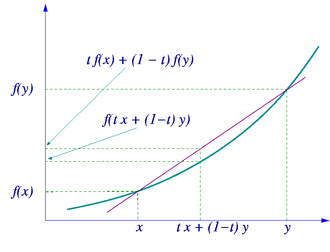
\includegraphics{images/convex_function_graph.png}
			\caption{Illustration fonction convexe [image de Wikipédia]}
			\label{fig:convexe_graph}
		\end{figure}	
		
		\paragraph*{Définition : (Fonction convexe)}
		Une fonction $f$ d'un intervalle réel $I \in \mathcal{C}$ est dite fonction convexe lorsque, $\forall (x,y)$ de $I$ tel que $(x,y) \in \mathcal{C}^2$ et tout $\alpha \in [0, 1]$  on a :
		
				
		\begin{equation}
			f(\alpha x + (1 - \alpha)y) \leq \alpha f(x) + (1 - \alpha)f(y)
			\label{eq_convexe-1}
		\end{equation}
		et si
		\begin{equation}
			f(\alpha x + (1 - \alpha)y) < \alpha f(x) + (1 - \alpha)f(y)
			\label{eq_convexe-2}
		\end{equation}
		on dit que la fonction est strictement convexe dans $\mathcal{C}$,  \cite{jtshiman:2021}\\\\
		Exemple: 
		%\begin{itemize}
			%\item[--] La fonction $ f(x) = x^2$ est convexe. 
			%\item[--] La fonction $ f(x) = x^T x$ est convexe.
			%\item[--] La fonction $ f(x) = x^T Ax$ est convexe, ssi A est symétrique semi-définie %positive.
		%\end{itemize}coulombeau2013math
	
		%\subsection{Extrema}	
		\paragraph*{Propriété d'une fonction dérivable : } (Extremum local) 
		Parmi les propriétés de dérivabilité il existe une qui est mise en relation avec l'effect qu'une fonction doit être convexe. énoncé ci-dessous \cite[][p. 212]{coulombeau2013math}.\\
		\begin{list}{+}{Soit $I \rightarrow  \mathbb{R} $ une fonction et $a$ un point de $I$.}
			\item  {On dit que $m$ est un \textbf{minimum local} de $f$ s'il existe $a > 0$ tel que $m$ soit le minimum de $f$ restreinte à $I \cap ] a-\alpha, a + \alpha [$. }
			\item On dit que $M$ est un \textbf{maximum local} de $f$ s'il existe $a > 0$ tel que $M$ soit le maximum de $f$ restreinte à $I \cap ] a-\alpha, a + \alpha [$. 
		\end{list} 
		
		Donc nous pouvons dire qu'une fonction convexe à un unique point minimum.
		
		 
	\subsubsection{\textbf{Développement limité}}\label{sec:dev_lim}
		En physique et en mathématiques, un développement limité (noté DL) d'une fonction en un point est une approximation polynomiale de cette fonction au voisinage de ce point, c'est-à-dire l'écriture de cette fonction sous la forme de la somme d'une fonction polynomiale et d'un reste négligeable au voisinage du point considéré \cite{coulombeau2013math}.
		
		Soit $f$ une fonction à valeurs réelles définie sur un intervalle $I$, et $x_0 \in I$. On dit que $f$ admet un développement limité d'ordre $n^2$ (abrégé par $DL_n$) en $x_0$, s'il existe $n + 1$ réels $a_0, a_1, \dots, a_n$  tels que la fonction ${\displaystyle R:I\to \mathbb {R} }$ définie par :
		$${\displaystyle f(x)=a_{0}+a_{1}(x-x_{0})+a_{2}(x-x_{0})^{2}+\dots+a_{n}(x-x_{0})^{n}+R(x)=\sum _{i=0}^{n}a_{i}(x-x_{0})^{i}+R(x)}$$
		vérifie : $R(x)$ tend vers $0$ lorsque $x$ tend vers $x_0$, et ce plus rapidement que le dernier terme de la somme, c'est-à-dire que :
		$$
			\lim _{{x\rightarrow x_{0}}}{\frac{R(x)}{(x-x_{0})^{n}}}=0. 
		$$
		
		La fonction reste $R(x)$ vérifiant ceci est notée $o((x – x0)^n)$ (selon la notation de Landau). On écrit donc :
		
		$$
			f(x)= \sum _{i=0}^{n}a_{i}(x-x_{0})^{i}+R(x) =\sum _{{i=0}}^{n}a_{i}(x-x_{0})^{i}+o((x-x_{0})^{n})
		$$
		
		%\begin{tabular}{r l}
			%\( f(x)\) & \( =\sum _{i=0}^{n}a_{i}(x-x_{0})^{i}+R(x)\) \\
			%& \(=\sum _{{i=0}}^{n}a_{i}(x-x_{0})^{i}+o((x-x_{0})^{n}) \)
		%\end{tabular}
		
		Il est fréquent d'écrire un développement limité en posant $x = x0 + h$ on aura:
		
		
		$$
			f(x_{0}+h)=\sum _{{i=0}}^{n}a_{i}h^{i}+o(h^{n})
		$$
		
		\paragraph*{Conséquences immédiates}
		\begin{itemize}
			\item Si $f$ admet un $DL_0$ en $x_0$, alors $a_0 = f(x_0)$. \cite{coulombeau2013math}
			\item Si $f$ admet un $DL_n$ en $x_0$, alors elle admet un $DL_k$ en $x_0$ pour tout entier $k < n$ \cite{coulombeau2013math}.
			\item Une condition nécessaire et suffisante pour que f admette un $DL_n$ en $x_0$ est l'existence d'un polynôme $P$ tel que $f(x) = P(x) + o((x – x_0)^n)$ \cite{coulombeau2013math}. S'il existe un tel polynôme $P$, alors il en existe une infinité d'autres, mais un seul d'entre eux est de degré inférieur ou égal à $n$ : le reste de la division euclidienne de $P(X)$ par $(X – x_0)^{n+1}$. On l'appelle la partie régulière, ou partie principale, du $DL_n$ de $f$ en $x_0$. %On identifie parfois, par abus de langage, le $DL_n$ avec sa partie régulière.
		\end{itemize}
		
		
			
		Le théorème de Taylor-Young assure \cite{coulombeau2013math} qu'une fonction $f$ dérivable n fois au point $x_0$ (avec ${\displaystyle n\geq 1}n\geq 1)$ admet un DLn en ce point :
		
		$$
			{\displaystyle f(x)=f(x_{0})+f'(x_{0})(x-x_{0})+{\frac {f''(x_{0})}{2!}}(x-x_{0})^{2}+\dots +{\frac {f^{(n)}(x_{0})}{n!}}(x-x_{0})^{n}+o((x-x_{0})^{n})}
		$$
		
		soit en écriture abrégée
		$$
			f(x)=\sum _{{i=0}}^{n}{\frac  {f^{{(i)}}(x_{0})}{i!}}(x-x_{0})^{i}+o((x-x_{0})^{n})
		$$
		
		Le développement d'ordre $0$ en $x_0$ revient à écrire que $f$ est continue en $x_0$ :
		
		$$
		{\displaystyle f(x)=f(x_{0})+o((x-x_{0})^{0})=f(x_{0})+o(1)}
		$$
		
		Le développement limité d'ordre 1 en $x_0$ revient à approcher une courbe par sa tangente en $x_0$ on parle aussi d'approximation affine :
		
		$$
		f(x)=f(x_{0})+f'(x_{0})\cdot (x-x_{0})+o(x-x_{0})
		$$
		
	%\subsubsection{Différentiabilité au sens de Fréchet} \label{sec:drv_frechet}
		%Soient $E$ un espace vectoriel normé, $F$ un espace vectoriel topologique séparé, $f$ une application de $E$ dans $F$ et $a$ un point de $E$. On abandonne la notation des vecteurs par des flèches dans ce paragraphe.
			
		%On dit que $f$ est différentiable en $a$ (au sens de Fréchet) s'il existe une application linéaire continue ${\displaystyle L:E\to f}$ telle que :
		%$$
		%	\forall h\in E\quad f(a+h)=f(a)+L(h)+o\left(\|h\|\right)
		%$$
		%ou, de manière équivalente :
			
		%$$
		%	\lim _{h\to 0}{\frac {f(a+h)-f(a)-L(h)}{\|h\|}}=0.
		%$$
			
		%Une telle application linéaire $L$ est alors unique.
		%L’opérateur $L$ est appelé différentielle de Fréchet (ou F-différentielle, ou Fréchet-différentielle) de $f$ au point $a$, et $f$ est dite Fréchet-différentiable (ou différentiable, ou différentiable au sens de Fréchet) au point $a$. La différentielle de $f$ au point $a$ est souvent notée $Df(a)$, la notation
		%$f'(a)$ est aussi utilisée.
	%\subsubsection{Fonctions dérivables}
		
	
	\subsubsection{\textbf{Gradient}}\label{sec:gradient}
		\paragraph*{Définition:}Le gradient d'une fonction de plusieurs variables en un certain point est un vecteur qui caractérise la variabilité de cette fonction au voisinage de ce point. Défini en tout point où la fonction est différentiable, il définit un champ de vecteurs, également dénommé gradient. Le gradient est la généralisation à plusieurs variables de la dérivée d'une fonction d'une seule variable.%\\ \\
		\paragraph*{Définition mathématique :} Dans un système de coordonnées cartésiennes, le gradient d'une fonction {$ f(x_{1},x_{2},\dots ,x_{n}$)} est le vecteur de composantes {$ \partial f/ \partial x_{i}\ (i=1,2,\dots ,n)$}, c'est-à-dire les dérivées partielles de $f$ par rapport aux coordonnées \cite{jtshiman:2021}.
		$${\nabla f(x)={
				\begin{bmatrix}
					{\frac {\partial f(x)}{\partial x_{1}}}\\
					\vdots \\
					{\frac {\partial f(x)}{\partial x_{n}}}
				\end{bmatrix}}} \in \mathbb{R}^n $$
		%\pagebreak
		\paragraph*{Gradient sous forme de développement limité:}
		\textit{Si une application admet un gradient en un point, alors on peut écrire ce développement limité du premier ordre (voir le point \ref{sec:dev_lim})}.
		
		$${ 
			f(x+h)=f(x)+\langle \nabla f(x)\mid h\rangle +o(h) 
		}$$ 
		ou 
		$$ {  
			f(x-h)=f(x)-\langle \nabla f(x)\mid h\rangle +o(h)
		}$$
		\textit{Numériquement, il est très intéressant de faire ensuite la demi-différence des deux développements pour obtenir la valeur du gradient et on note que celui-ci ne dépend pas en fait de la valeur de la fonction au point $x : f (x)$. Cette formule a l'avantage de tenir compte des gradients du 2e ordre et est donc beaucoup plus précise et numériquement robuste. L'hypothèse est, en pratique, de connaitre les valeurs "passé" et "futur" de la fonction autour d'un petit voisinage du point $x$}\cite{jtshiman:2021}.\\
		\paragraph*{Définition numérique:}
		Une fonction multivariée (à variable vectorielle)
		$ f(x)	: \mathbb{R}^n \rightarrow \mathbb{R} : x \rightarrow f(x) $ définie sur un ouvert $O \in \mathbb{R}^n$ est dite dérivable (au sens de Fréchet, voir le point \ref{sec:drv_frechet}) en $x$ ssi il existe un vecteur noté $\nabla f(x) \in \mathbb{R}^n$ tel que
		\begin{equation}
			f(x+h) = f(x) + \nabla f(x)^{T}h + o(||h||)
		\end{equation}
		
		$\nabla f(x) \in \mathbb{R}^n$ et où l’on a posé que le reste $o(||h||) = ||h||\epsilon (h) \in \mathbb{R}^n$, avec $h \in \mathbb{R}^n$ 
		\begin{center}
			$\epsilon (h): \mathbb{R}^n\rightarrow \mathbb{R}, \qquad \lim\limits_{||h|| \rightarrow 0} \epsilon(h)=0$.
		\end{center} 
		Le vecteur $\nabla f(x)$ est unique et nommé \textbf{gradient} de $f(x)$ en $x$.
		Le gradient s’adresse aux fonctions scalaires à variables vectorielles.
		\paragraph*{A propos de la notation \textbf{$o(||h||)$}:}
		La notation de Bachmann-Landau $o(||h||)$ traduit le comportement d’une fonction de $h$ qui tend vers $0$ d’un ordre de grandeur plus vite que $||h||$.\\\\
		Elle est infiniment plus petit que $h$ dans le voisinage de $0$
		
		
		
			
	\subsubsection{\textbf{Hessienne}}
		\paragraph*{Définition mathématique:}
		Étant donnée une fonction ${f}$ à valeurs réelles
		
		$${ f:\mathbb{R}^{n}\to \mathbb {R} ;(x_{1},...,x_{n})\mapsto f(x_{1},...,x_{n})}$$
		dont toutes les dérivées partielles secondes existent, le coefficient d'indice ${ i,j}$ de la \textbf{matrice hessienne\footnote{En mathématiques, la matrice hessienne (ou simplement la hessienne) d'une fonction numérique $f$ est la matrice carrée, notée $H(f)$, de ses dérivées partielles secondes.}} ${H(f)}$ vaut ${H_{ij}(f)={\frac {\partial ^{2}f}{\partial x_{i}\partial x_{j}}}}$.\\
		Autrement dit,
		$$
		{ H(f)={
			\begin{bmatrix}{
				\frac {\partial ^{2}f}{{\partial x_{1}}^{2}}}&{\frac {\partial ^{2}f}{\partial x_{1}\partial x_{2}}}&\cdots &{\frac {\partial ^{2}f}{\partial x_{1}\partial x_{n}}}\\
				{\frac {\partial ^{2}f}{\partial x_{2}\partial x_{1}}}&{\frac {\partial ^{2}f}{{\partial x_{2}}^{2}}}&\cdots &{\frac {\partial ^{2}f}{\partial x_{2}\partial x_{n}}}\\
				\vdots &\vdots &\ddots &\vdots \\
				{\frac {\partial ^{2}f}{\partial x_{n}\partial x_{1}}}&{\frac {\partial ^{2}f}{\partial x_{n}\partial x_{2}}}&\cdots &{\frac {\partial ^{2}f}{{\partial x_{n}}^{2}}}
			\end{bmatrix}}} .
		$$
		
		\paragraph*{Définition numérique:}
		Supposons que $f : \mathbb{R}^{n} \to \mathbb{R}$ définie sur un ouvert $\mathcal{O} \in \mathbb{R}^{n}$. La fonction $f(x)$ est dite 2
		fois continûment dérivable (au sens de Fréchet??) si en tout $x \in \mathcal{O}$ on a
		
		\begin{equation}
			f(x + h) = f(x)+\nabla f(x)^Th + \frac{1}{2}h^T\nabla^2f(x)h+o(||h||^2)
		\end{equation}
		avec$\nabla f(x)\in \mathbb{R}^{n\times n}$ et où on a posé que le reste 
		$ o(||h||^2) =||h|| \epsilon(h) \in \mathbb{R} $ avec 
		$\lim\limits_{||h|| \to 0} \epsilon(h) = 0 $
		La matrice carrée symétrique $\nabla^2 f(x)$ appelée \textbf{Hessien} de $f(x)$ en $x$. Remarque :
		
		$$
			\lim\limits_{||h|| \to h} \frac{o(||h||^2)}{||h||} = 0  \in \mathbb{R}
		$$
		La Hessienne s’adresse aux fonctions scalaires à variables vectorielles.
	%---------------------------------------------------
	%	JACOBIENNE
	%---------------------------------------------------			
	\subsection{Échantillonnage (statistique)} % \& probabilité bayésienne}

		%\subsubsection{Échantillonnage (statistique)}
		
		En statistiques, l'échantillonnage est la sélection d'un sous-ensemble (un échantillon statistique ) d'individus au sein d'une population statistique pour estimer les caractéristiques de l'ensemble de la population. 
		
		
		Sur un échantillon, on peut calculer différents paramètres statistiques de position (moyenne, etc.) ou de dispersion (écart type, etc.) issus de la statistique descriptive, de la même manière que l'on peut déterminer des paramètres statistiques d'une population par son recensement exhaustif.
		
		On peut également déduire des propriétés de la population à partir de celles de l'échantillon par inférence statistique. D'après la loi des grands nombres, plus la taille de l'échantillon augmente, plus ses propriétés seront proches de celle de la population. En particulier, on peut estimer une probabilité sur les individus d'une population par la fréquence observée sur un échantillon si sa taille est suffisamment grande. 
		
		Cette méthode présente plusieurs avantages : une étude restreinte sur une partie de la population, un moindre coût, une collecte des données plus rapide que si l'étude avait été réalisé sur l'ensemble de la population, la réalisation de contrôles destructifs, etc.
		
		\begin{list}{$\triangleright$ }{On peut procéder de différentes manières pour collecter les données de l'échantillon, il existe en effet plusieurs méthodes d'échantillonnage \cite{sarndal2003model} :}
			%\textbf
			\item  \textbf{Échantillonnage aléatoire et simple }: le tirage des individus de l'échantillon est aléatoire, c'est-à-dire que chaque individu a la même probabilité d'être choisi, et simple, c'est-à-dire que les choix des différents individus sont réalisés indépendamment les uns des autres.
			%L'échantillonnage aléatoire simple peut être vulnérable aux erreurs d'échantillonnage car le caractère aléatoire de la sélection peut donner un échantillon qui ne reflète pas la composition de la population. 
			
			\item  \textbf{Échantillonnage systématique }: le premier individu est choisi de manière aléatoire, puis les suivants sont déterminés à intervalle régulier. Par exemple, dans un verger, on choisit au hasard le 7e pommier, puis les 27e, 47e, 67e, etc.
			
			\item  \textbf{Échantillonnage stratifié }: on subdivise la population en plusieurs parties avant de prendre l'échantillon1.
			
			\item \textbf{Échantillonnage par quotas }: la composition de l'échantillon doit être représentative de celle de la population selon certains critères jugés particulièrement importants. On utilise cette méthode pour réaliser les sondages d'opinions.
		\end{list}

	
		\subsubsection{\textbf{La collecte de données} }
		
		La collecte de données est le processus de collecte et de mesure des informations sur des variables ciblées dans un système établi, qui permet ensuite de répondre aux questions pertinentes et d'évaluer les résultats.
		
		\begin{list}{--}{Une bonne collecte de données implique :}
			\item Suivre le processus d'échantillonnage défini
			\item Garder les données dans l'ordre du temps
			\item Noter les commentaires et autres événements contextuels
			\item Enregistrement des non-réponses
		\end{list}
		
		\paragraph*{Erreur d'échantillonnage :}
		Dans les statistiques, les erreurs d'échantillonnage se produisent lorsque les caractéristiques statistiques d'une population sont estimées à partir d'un sous-ensemble, ou échantillon, de cette population. Étant donné que l'échantillon n'inclut pas tous les membres de la population, les statistiques de l'échantillon (souvent appelées estimateurs), telles que les moyennes et les quartiles, diffèrent généralement des statistiques de l'ensemble de la population (appelées paramètres ). La différence entre la statistique d'échantillon et le paramètre de population est considérée comme l'erreur d'échantillonnage \cite{sarndal2003model}. 
	
	
	
		
	%\subsubsection{Généralité sur l'analyse bayésienne}
		%La statistique bayésienne est une théorie dans le domaine des statistiques basée sur l' interprétation bayésienne de la probabilité où la probabilité exprime un degré de croyance en un événement. Le degré de croyance peut être basé sur des connaissances antérieures sur l'événement, telles que les résultats d'expériences précédentes, ou sur des croyances personnelles sur l'événement. Cela diffère d'un certain nombre d'autres interprétations de la probabilité , telles que l' interprétation fréquentiste qui considère la probabilité comme la limite de la fréquence relative d'un événement après de nombreux essais [??].
		
		%Les statistiques bayésiennes portent le nom de Thomas Bayes qui a formulé un cas spécifique du théorème de Bayes dans un article publié en 1763.
		
		
		
		%\begin{thm}[Théorème de Bayes] Le théorème de Bayes est utilisé dans les méthodes bayésiennes pour mettre à jour les probabilités, qui sont des degrés de croyance, après avoir obtenu de nouvelles données. Compte tenu de deux événements $A$  et $B$, la probabilité conditionnelle de $A$ étant donné que $B$ est vrai s'exprime comme suit  :
			%\begin{equation}
				%\mathbb{P}(A|B) = \frac{\mathbb{P}(B|A) \mathbb{P}(A)}{\mathbb{P}(B)}
			%\end{equation}
			
		%\end{thm}
	
		%où $\mathbb{P}(B) \ne 0$ Bien que le théorème de Bayes soit un résultat fondamental de la théorie des probabilités , il a une interprétation spécifique dans les statistiques bayésiennes \cite[][]{antoine2018apprentissage}.

		
%#############################################################################
%
%              						CHAPTER 
%
%#############################################################################


%\textcolor{cyan}{\chapter{Apprentissage automatique : Modélisation et Classification }}
	%\section{Généralité}
	
	\pagebreak
\section{Concepts de la modélisation et classification des données}
	\subsection{Introduction}
	\subsubsection{Les ingrédients d'apprentissage}
		Résoudre un problème d'apprentissage, c'est d'abord le comprendre, c'est-à-dire discuter longuement avec les experts du domaine concerné pour identifier quelles sont les "entrées", les  "sorties" ou résultats désirés, les connaissances disponibles, les particularités des données, par exemple: valeurs manquantes, taux de bruit dans les mesures des attributs de description, proportions des classes, stationnarité ou pas de l'environnement. 
		C'est aussi réaliser un gros travail de \textit{préparation des données}: nettoyage, ré-organisation, enrichissement, intégration avec d'autres sources de données, etc.Ces étapes de compréhension du problème, de préparation des données, de mise au point du protocole d'apprentissage et des mesures d'évaluation des résultats, prennent, et de loin, la plus grande partie du temps pour (tenter de) résoudre un problème d'apprentissage \cite{antoine2018apprentissage}. 
		Nous avons toujours tendance à largement sous-estimer ces étapes et à vouloir se concentrer uniquement sur la phase excitante de l'essai de méthodes d'apprentissage sur des données supposées bonnes à la consommation. 
		%\subsubsection{Algorithme qui apprennent}
	
	
	\subsubsection{Concepts de la modélisation}\label{sec:modelisation}
	La modélisation est la conception et l'utilisation d'un \textit{modèle}. Selon son objectif et les moyens utilisés, la modélisation est dite mathématique, géométrique, 3D, empirique, etc. 
	En informatique, la modélisation permet de concevoir l'architecture globale d'un système d'information, ainsi que l'organisation des informations à l'aide de la modélisation des données ;
	
	\paragraph*{Modèle (informatique):} En informatique, un modèle a pour objectif de structurer les informations et activités d'une organisation : données, traitements, et flux d'informations entre entités.
	
	\paragraph*{Modèle (mathématique):} Un modèle mathématique est une description d'un système utilisant des concepts et un langage mathématiques.
	
	Un modèle peut aider à expliquer un système et à étudier les effets de différents composants, et à faire des prédictions sur le comportement.
	
	\subsubsection*{Modèles non paramétriques}
	
	
	\Eg: Prenons l'exemple de données décrites dans l'espace d'entrée $\mathcal{X} = \mathbb{R}^n$ avec $n$ variables réelles et supposons-les étiquetées par $\times$ ou par $\bullet$. On cherche donc une fonction de décision $h$, appelée hypothèse ou modèle, telle qu'elle soit capable d'étiqueter toute entrée 
	$x \in \mathcal{X}, h: x \rightarrow \{\times,\bullet\}$. Reste à définir l'espace des hypothèses ou modèles $\mathcal{H}$ que l'on est prêt à considérer.
	
	Toujours en considérant le problème de prédiction basique (présenté ci-dessus), on pourrait définir une hypothèse par une procédure qui examine les trois plus proches voisins du point à étiqueter $x$ et qui choisit l'étiquette majoritaire parmi ces trois points pour étiqueter $x$. Il n'y a évidemment plus de paramètres pour définir les modèles possibles \cite{antoine2018apprentissage}.
	
	Un \textbf{modèle non paramétrique} est construit selon les informations provenant des données. Dans \cite{bishop2006pattern, antoine2018apprentissage} il est expliqué que : La régression non paramétrique exige des tailles d'échantillons plus importantes que celles de la régression basée sur des modèles paramétriques parce que les données doivent fournir la structure du modèle ainsi que les estimations du modèle.
	
	Un \textbf{modèle paramétrique} est, s'il est approximativement valide, plus puissant qu'un modèle non paramétrique, produisant des estimations d'une fonction de régression qui ont tendance à être plus précises que ce que nous donne l'approche non paramétrique \cite{matloff2017statistical}. Cela devrait également se traduire par une prédiction plus précise. 
	
	
	
	\begin{list}{--}{Selon \cite{antoine2018apprentissage}, nous pouvons construire un modèle d'apprentissage, ou l'espaces des hypothèses d'apprentissage, par: }
		\item La classification
		\item La régression
		\item Les distributions de probabilités
		\item Les arbres de décisions
		\item Les réseaux bayésiens 
		\item Etc.
	\end{list}

	La table suivante présente d'abord les qualités des différentes représentations des hypothèses en fonction des critères cités ci-dessus.
	

	%\parbox[t]{2mm}{\multirow{3}{*}{\rotatebox[origin=c]{90}{rota}}} 
	\begin{center}
		\begin{tabular}{l|cccccc}
			& \rotatebox[origin=c]{90}{Fonctions séparatrices}
			&  \rotatebox[origin=c]{90}{Distributions de probabilités}
			& \rotatebox[origin=c]{90}{Arbres de décision }
			& \rotatebox[origin=c]{90}{Hiérarchies de concepts}
			& \rotatebox[origin=c]{90}{Réseaux bayésiens } 
			& \rotatebox[origin=c]{90}{Chaînes de Markov}\\
			\hline
			
			Concept & $\surd$ &$\surd$ &$\surd$ &$\surd$ & --&-- \\
			Classes multiples &$\surd$ & $\surd$ &$\surd$ &$\surd$ &--&-- \\
			Ontologies & --&-- & $\surd$&$\surd$ & --&-- \\
			Régression &-- &$\surd$ & $\surd$&-- &-- &-- \\
			Évolutions temporelles &-- &$\surd$ &-- &-- &-- & $\surd$\\
			Apprentissage non supervisé & $\surd$ &$\surd$ &$\surd$ &$\surd$ &-- &-- \\
			Données continues & $\surd$ &$\surd$ &$\surd$ &-- &-- &$\surd$  \\
			Connaissances relationnelles  & & & & $\surd$  & $\surd$  &-- \\
			Degré de certitude &-- &$\surd$ &-- &-- &$\surd$ &$\surd$ \\
			Degré d'imprécision &-- &$\surd$ &-- &-- &$\surd$ &-- \\
			Transparence, intelligibilité &-- &-- &-- &$\surd$ &$\surd$ &$\surd$ \\
			%& & & & \\
			%& & & & \\
			
			
		\end{tabular}
	\end{center}

	
	
	\subsubsection*{Entraînement du modèle}
	
	Tout modèle, où toutes les informations nécessaires ne sont pas disponibles, contient certains paramètres qui peuvent être utilisés pour adapter le modèle au système qu'il est censé décrire. Si la modélisation est effectuée par un réseau de neurones artificiels ou un autre apprentissage automatique, l'optimisation des paramètres est appelée \textbf{entraînement} (en anglais : \textbf{training}), tandis que l'optimisation des hyperparamètres du modèle est appelée \textbf{réglage} (en anglais: \textbf{tuning}) et utilise souvent la validation croisée \cite{goodfellow2016deep}. Dans une modélisation plus conventionnelle à travers des fonctions mathématiques explicitement données, les paramètres sont souvent déterminés par ajustement de courbe (voir le point ??).
	
	
	Une partie cruciale du processus de modélisation consiste à évaluer si oui ou non un modèle mathématique donné décrit un système avec précision. Il peut être difficile de répondre à cette question car elle implique plusieurs types d'évaluation différents.
	
	

	\subsection{Les problèmes de régressions} \label{sec:regression_problem}
	
	L'algorithme d'apprentissage automatique est défini comme un algorithme capable d'améliorer les performances d'un programme informatique à certaines tâches via l'expérience est quelque peu abstraite. Pour rendre cela plus concret, Une des méthode d'apprentissage automatique basique est \emph{la régression linéaire}\cite{goodfellow2016deep}.
	
	Dans la modélisation statistique, l'analyse de régression est un ensemble de processus statistiques permettant d'estimer les relations entre une variable dépendante et une ou plusieurs variables indépendantes [??].\\
	En statistique, la régression linéaire est une approche linéaire pour modéliser (voir le point \ref{sec:modelisation}) la relation entre une réponse scalaire et une ou plusieurs variables explicatives (également appelées variables dépendantes et indépendantes). Le cas d'une variable explicative est appelé régression linéaire simple; pour plus d'un, le processus est appelé régression linéaire multiple.
	
	Dans la régression linéaire, les relations sont modélisées à l'aide de \textit{fonctions prédictives}\footnote{En statistique et en apprentissage automatique, une fonction de prédicteur linéaire est une fonction linéaire d'un ensemble de coefficients et de variables explicatives, dont la valeur est utilisée pour prédire le résultat d'une variable dépendante.} linéaires dont les paramètres de modèle inconnus sont estimés à partir des données \cite{matloff2017statistical}. De tels modèles sont appelés modèles linéaires.
	
	La régression linéaire a de nombreuses utilisations pratiques. Si l'objectif est la prédiction, la prévision ou la réduction des erreurs, la régression linéaire peut être utilisée pour ajuster un modèle prédictif à un ensemble de données observées de valeurs de la réponse et de variables explicatives \cite{darlington2016regression}. Après avoir développé un tel modèle, si des valeurs supplémentaires des variables explicatives sont collectées sans valeur de réponse d'accompagnement, le modèle ajusté peut être utilisé pour faire une prédiction de la réponse.
	
	Dans ce type de tâche, le programme informatique est invité à prédire une valeur numérique à partir d'une entrée donnée. Pour résoudre cette tâche, l'algorithme d'apprentissage est invité à sortir une fonction $f : \mathbb{R}^n \rightarrow \mathbb{R}$. Ce type de tâche est similaire à la \textbf{classification}, sauf que le format de sortie est différent \cite{goodfellow2016deep}.
	
	
	
	
	\subsubsection{Le cas de la régression linéaire}
		On appelle problèmes de régression de tels problèmes, dans lesquels la sortie est numérique, généralement un vecteur de réels, supposé dépendre de la valeur d'un certain nombre de facteurs en entrée\cite{matloff2017statistical}.
		
		\begin{figure}[hth]%bth
			\centering
			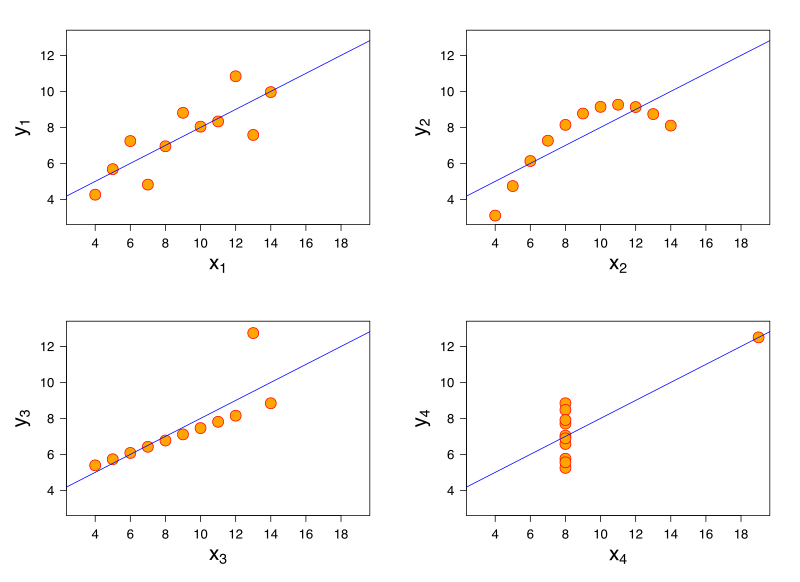
\includegraphics[width=\textwidth]{images/linear_regression_quartet.png}
			\caption{Images illustrant l'efficacité de la régression linéaire sur plusieurs type de modèle [image Wikipédia]
			}
			\label{fig:linear_regression_quartet}
		\end{figure}
		
		Le vecteur d'entrée $x = (x_1,x_2,...,x_n)^T$ est souvent appelé variable indépendante, tandis que le vecteur de sortie $y$ est appelé variable dépendante. On formalise le problème en supposant que la sortie résulte de la somme d'une fonction déterministe $f$ de l'entrée et d'un bruit aléatoire :
		\begin{equation}
			y = f(x) + \epsilon
		\end{equation}
	
		où $f(x)$ est la fonction inconnue que nous souhaitons approcher par un estimateur $h(x|w)$, où $h$ est défini à l'aide d'un vecteur $w$ de paramètres\cite{alpaydin2010introduction}.\\
		Si l'on suppose que le bruit $\epsilon$ est nulle et de variance constante $\sigma^2$, c'est-à-dire $ \epsilon = \mathcal{N}(0,\sigma^2)$, alors, en plaçant notre estimateur $h(\cdot)$ à la place de la fonction inconnue, on devrait avoir la densité conditionnelle réelle $p(y|x)$ vérifiant :
		\begin{equation}
			p(y|x) = \mathcal{N}(h(x|w),\sigma^2)
		\end{equation}
		
		On peut estimer le vecteur de paramètres $w$ grâce au principe de maximisation de la vraisemblance. On suppose que les couples $(x_t, y_t)$ de l'échantillon d'apprentissage sont tirés par tirages indépendants d'une distribution de probabilités jointes inconnue $p(x, y)$, qui peut s'écrire :
		
		$$
			p(y|x) = p(y|x)p(x)
		$$
		où $p(y|x)$ est la probabilité de la sortie étant donnée l'entrée et $p(x)$ est la densité de probabilité sur les entrées \cite{matloff2017statistical}.
		
		Étant donné un échantillon d'apprentissage $S = \langle (x_t,y_t) \rangle_{1\leq t\leq m} $ supposé tiré de manière indépendante et identiquement distribuée.
		Maximiser l'expression résultante revient alors à minimiser la somme de carrés des erreurs (SCE):
		\begin{equation}\label{eq:sce_1}
			SCE(w|\mathit{S}) = \frac{1}{2} \sum_{{t=1}}^{m}{ [ y_t - h(x_t|w) ]^2}	
		\end{equation}
		
	%%%\subsubsection*{La régression non linéaire ou multiple}
		%\lipsum[2]
	\subsubsection{Le cas de la régression générale}
		La plupart des modèles de régression proposent que $Y_{i}$ est une fonction de $X_{i}$ et $w$, avec $\epsilon_{i}$ représentant un terme d'erreur additif ou bruit statistique aléatoire qui peut remplacer des déterminants non modélisés de $Y_{i}$ :
		\begin{equation}
			{\displaystyle Y_{i}=f(X_{i},w )+\epsilon_{i}}
		\end{equation}
	
		L'objectif est d'estimer la fonction ${\displaystyle f(X_{i},w )}$ qui correspond le mieux aux données.
		
		Pour effectuer une analyse de régression, la forme de la fonction $f$ doit être spécifié. Parfois, la forme de cette fonction est basée sur la connaissance de la relation entre $Y_{i}$ et $X_{i}$. 
		Si ces connaissances ne sont pas disponibles, un formulaire souple ou pratique pour $f$ est choisi. Par exemple, une simple régression univariée peut proposer
		 $${\displaystyle f(X_{i},w )= w_{0}+ w_{1}X_{i}}$$
		ou
		 $${\displaystyle Y_{i}= w_{0}+ w_{1}X_{i}+e_{i}}$$
		être une approximation raisonnable du processus statistique générant les données.
		 
		 Différentes formes d'analyse de régression fournissent des outils pour estimer les paramètres. $w$. Par exemple, les moindres carrés trouvent la valeur de $w$ qui minimise la somme des carrés des erreurs \cite{deepa2021ai} $${\sum _{i}(Y_{i}-f(X_{i},w ))^{2}}$$ 
		 
		 Étant donné un ensemble de données ${\displaystyle \{y_{i},\,x_{i1},\ldots ,x_{ip}\}_{i=1}^{n}}$ de $n$ unités statistiques, un modèle de régression linéaire suppose que la relation entre la variable dépendante $y$ et le vecteur $p$ des régresseurs $x$ est linéaire. Cette relation est modélisée par un terme de perturbation ou une variable d'erreur $\epsilon$ : une variable aléatoire non observée qui ajoute du "bruit" à la relation linéaire entre la variable dépendante et les régresseurs. Ainsi le modèle prend la forme
		 
		$${\displaystyle y_{i}=w _{0}+w _{1}x_{i1}+\cdots +w _{n}x_{in}+\varepsilon _{i}=\mathbf { x} _{i}^{\mathsf {T}}{\boldsymbol {w }}+\varepsilon_{i},\qquad avec \quad i=1,\ldots ,n,}
		$$
		
		Souvent, ces $n$ équations sont empilées et écrites en notation matricielle comme
		
		$$
		{\displaystyle \mathbf {y} =X{\boldsymbol {w}}+{\boldsymbol {\varepsilon}},\,}
		$$
		
		où
		
		$
		\mathbf{y} ={\begin{pmatrix}y_{1}\\y_{2}\\\vdots \\y_{n}\end{pmatrix}},\quad
		{\displaystyle 
			X={
				\begin{pmatrix}
					\mathbf {x} _{1}^{\mathsf {T}}\\
					\mathbf {x} _{2}^{\mathsf {T}}\\
					\vdots \\
					\mathbf {x} _{n}^{\mathsf {T}}
				\end{pmatrix}}={
				\begin{pmatrix}
					1&x_{11}&\cdots &x_{1p}\\
					1&x_{21} &\cdots &x_{2p}\\
					\vdots &\vdots &\ddots &\vdots \\
					1&x_{n1}&\cdots &x_{np}
				\end{pmatrix}},} \quad
		{\displaystyle {\boldsymbol {\mathcal{W}}}={
				\begin{pmatrix}
					w _{0}\\
					w _{1}\\
					w _{2}\\
					\vdots \\
					w _{p}
				\end{pmatrix}},\quad 
		{\boldsymbol {\varepsilon }}={
			\begin{pmatrix}\varepsilon _{1}\\
				\varepsilon _{2}\\
				\vdots \\
				\varepsilon _{ n}
			\end{pmatrix}}.}$ \\
	
		$\mathbf{y}$ est un vecteur de valeurs observées ${\displaystyle y_{i}\ (i=1,\ldots ,n)}$ de la variable appelée variable mesurée ou variable dépendante.
		
		$X$ peut être vu comme une matrice de vecteurs-lignes $\mathbf {x} _{i}$ ou de vecteurs-colonnes à $n$ dimensions $X_{j}$, appelées régresseurs, variables explicatives, variables d'entrée, variables prédictives ou variables indépendantes. La matrice $X$ est parfois appelée la matrice de conception. 
		
		${\boldsymbol {w}}$ est un vecteur de paramètre de dimension $(p+1)$, où $w _{0}$ est le terme d'interception, s'il n'est pas inclus dans le modèle ${\boldsymbol {w}}$ est de dimension $p$. Ses éléments sont appelés coefficients de régression \cite{antoine2018apprentissage}. 
		En régression linéaire simple, $p = 1$, et le coefficient est appelé \textbf{pente} de régression.\\
		L'estimation statistique et l'inférence dans la régression linéaire se concentrent sur $w$. Les éléments de ce vecteur de paramètres sont interprétés comme les dérivées partielles de la variable dépendante par rapport aux différentes variables indépendantes \cite{darlington2016regression}.
		
		En définissant les vecteurs  et matrice ci dessous, ${\boldsymbol X}$, ${\boldsymbol w}$ et ${\boldsymbol y}$ (avec ${S_y = y}$) \cite{antoine2018apprentissage}; le critère de la somme des carrées des erreurs s'écrit alors:
		\begin{equation}\label{eq:sce_2}
			SCE(w|\mathit{S}) = \frac{1}{2} ({\boldsymbol S_y }- \mathbf{X}\boldsymbol w)^{\mathsf{T}}({ \boldsymbol S_y }- \mathbf{X} \boldsymbol w)
		\end{equation}  
		Il suffit de prendre la dérivée de la somme des carrés des erreurs (équation \ref{eq:sce_1}) par rapport à $w$, qui est maintenant remplacer par $w$, pour obtenir les équations: 
		$$
			\frac{\partial SCE}{\partial w} = -{\boldsymbol X}^T({\boldsymbol S_y }- \mathbf{X} \boldsymbol w)
		$$
		
		$$
		\frac{\partial^2 SCE}{\partial^2 w \partial^2 w^T} = -{\boldsymbol X}^T{\boldsymbol X}
		$$
		
		En supposant que la matrice $X$ est non singulière, et donc que $X^TX$ est positive définie, et en posant que la dérivée première est nulle, on obtient :
		
		
		\begin{equation}
			{X^{T} Xw =  X^{T} S_y}
		\end{equation}
		\begin{tabular}{lr}
			
		\end{tabular}
	
		à partir de quoi on peut calculer l'unique solution par: 
		\begin{equation}
			\hat{w} = {(X^{T} X)^{-1} X^{T} S_y}
		\end{equation}
		La valeur $\hat{y}$ prédite pour une entrée $x_n$ est donc : 
		$$
			\hat{y} = \hat{w}\cdot x_n = {(X^{T} X)^{-1} X^{T} S_y}x_n 
		$$ 
		
		
		%Un modèle de régression linéaire ajusté peut être utilisé pour identifier la relation entre une seule variable prédictive $x_j$ et la variable de réponse $y$ lorsque toutes les autres variables prédictives du modèle sont "maintenues fixes". Plus précisément, l'interprétation de $\beta_j$ est la variation attendue de $y$ pour une variation d'une unité de $x_j$ lorsque les autres covariables sont maintenues fixes, c'est-à-dire la valeur attendue de la dérivée partielle de $y$ par rapport à $x_j$. Ceci est parfois appelé l'effet unique de $x_j$ sur $y$. En revanche, l'effet marginal de $x_j$ sur $y$ peut être évalué à l'aide d'un coefficient de corrélation ou d'un simple modèle de régression linéaire reliant uniquement $x_j$ à $y$; cet effet est la dérivée totale de $y$ par rapport à $x_j$.
			
		%\subsection{La régression linéaire simple}
			%\lipsum[3]
		%\subsection{La régression linéaire multivarié}
			%\subsubsection{Droite de régression} 
			%\subsubsection{Variance, Covariance, \& Corrélation}
		%\subsection{La fonction prédictif \& d'erreur}
			%\lipsum[1]
			
	\begin{figure}[hth]%bth
		\centering
		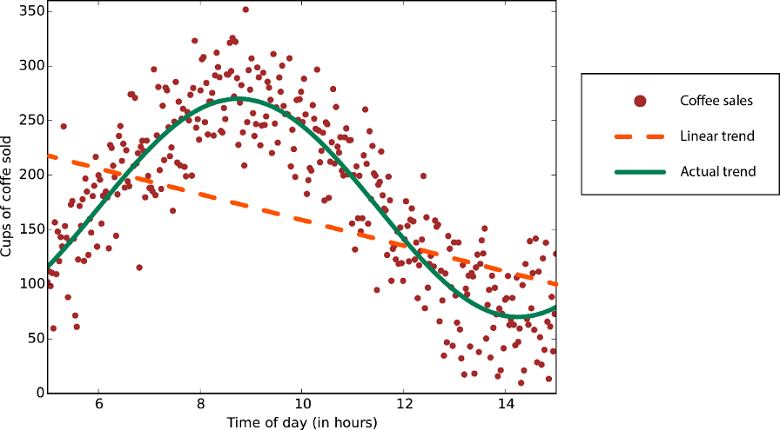
\includegraphics[width=\textwidth]{images/nonlinear-trend.png}
		\caption{ L'efficacité de la régression non linéaire par rapport \`{a} une régression linéaire..}
		\label{fig:nonlinear_trend}
	\end{figure}

	\paragraph*{}
	La régression linéaire multiple est une généralisation de la régression linéaire simple au cas de plus d'une variable indépendante, et un cas particulier des modèles linéaires généraux, limités à une variable dépendante.
	
	
	\subsection{Les problèmes de classifications} \label{sec:classificarion_problem}
		En apprentissage automatique, les classifieurs linéaires sont une famille d'algorithmes de classement statistique. Le rôle d'un classifieur est de classer dans des groupes (des classes) les échantillons qui ont des propriétés similaires, mesurées sur des observations. Un classifieur linéaire est un type particulier de classifieur, qui calcule la décision par combinaison linéaire des échantillons \cite{antoine2018apprentissage}.
		
		\begin{figure}[bth]%bth
			\centering
			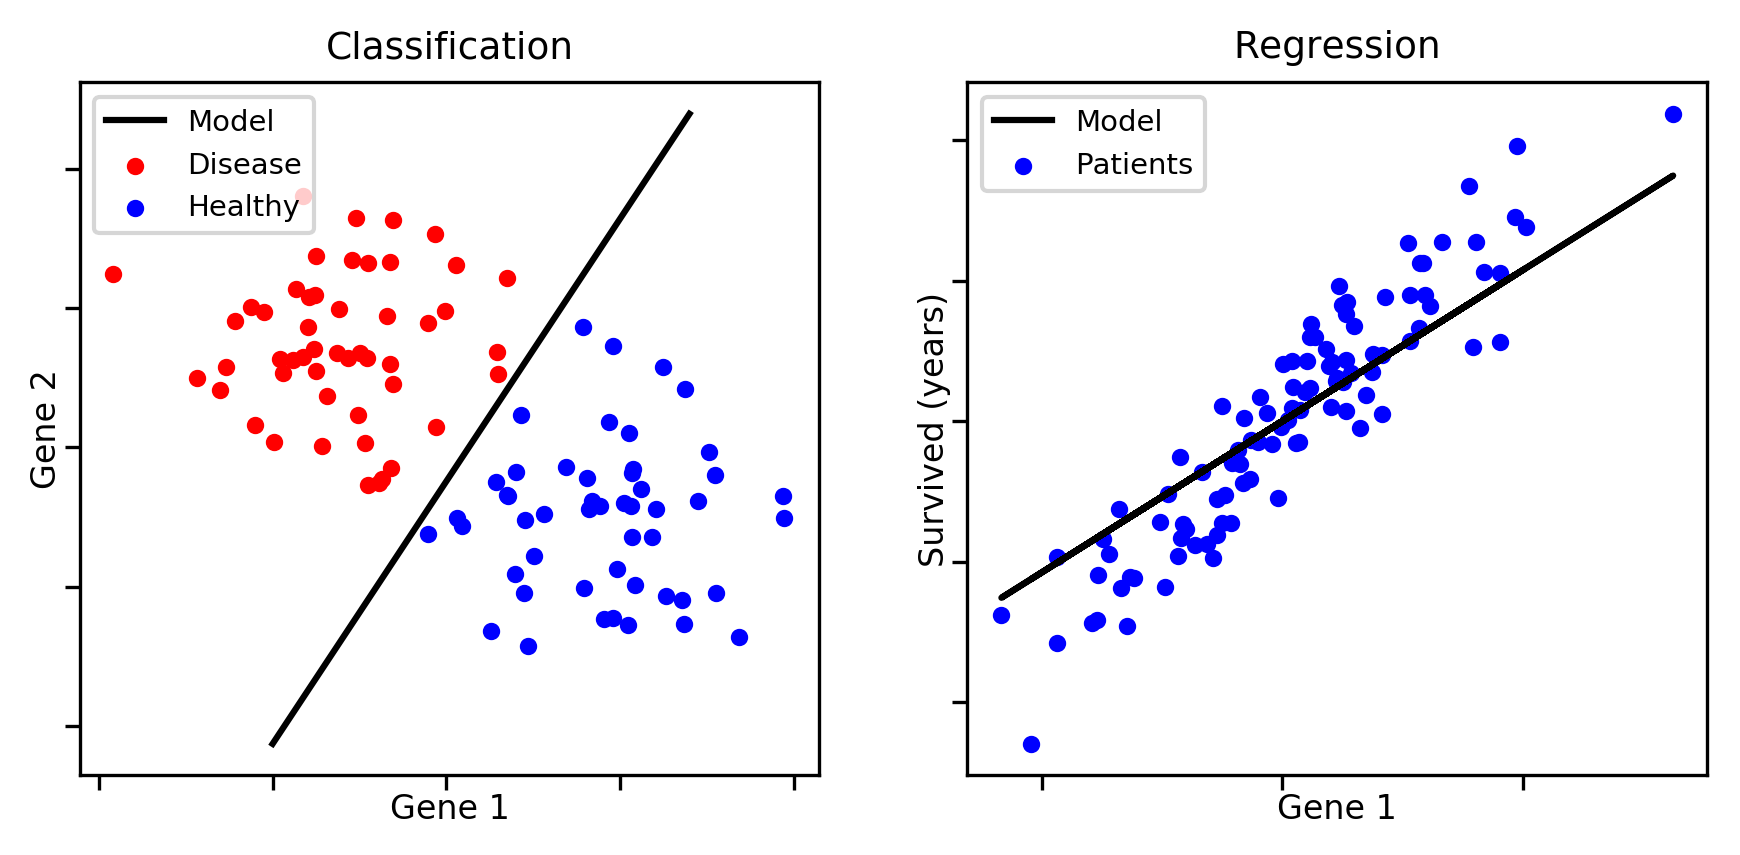
\includegraphics[width=15cm]{images/classification_vs_regression.png}
			\caption{Classification vs régression \cite{ml2008python}
			}
			\label{fig:class_vs_reg}
		\end{figure}
		
		Nous nous plaçons dans le cadre où la variable dépendante ou à prédire prend ses valeurs dans un ensemble fini que l'on associe généralement à un ensemble de classes. A la différence de la régression linéaire où l’ensemble de valeurs à prédire est infini.
		
		Lorsque l'on se place dans un espace de représentation euclidien, on peut librement faire des hypothèses sur la géométrie des classes ou sur celles de leurs surfaces séparatrices. La plus simple d'entre elles est de supposer que deux classes peuvent être séparées par une certaine surface, définie par une équation; les paramètres qui régissent cette équation sont alors les variables à apprendre.
		
		Le nombre de paramètres à calculer est minimal si l'on suppose cette surface linéaire; aussi est-ce l'hypothèse qui prévaut souvent, en particulier lorsque l'échantillon de données est de taille réduite par rapport à la dimension de l'espace d'entrée, d'autant qu'elle permet de mener des calculs faciles et de visualiser précisément le résultat obtenu \cite{sarkar2017practical}.
		
		Dans $\mathbb{R}^n$, une surface linéaire est un hyperplan $A$, défini par l'équation :
		$$ 
			a_0  + a^Tx = 0
		$$
		
		avec $a$ vecteur de dimension $n$ et $a_0$ scalaire. Si deux classes $\mathcal{C}_1$ et $\mathcal{C}_2$ sont \textit{séparables} par $A$, tous les points de la première classe sont par exemple tels que :
		
			\begin{equation}\label{eq:x_case_c1}
			 x \in \mathcal{C}_1 \implies a_0 + a^Tx > 0
			\end{equation}
		
		et ceux de la seconde vérifient alors :
		
			\begin{equation}\label{eq:x_case_c2}
				x \in \mathcal{C}_2 \implies a_0 + a^Tx \leq 0
			\end{equation}
			
		
		Dans un espace de dimension $d = 1$, une séparation linéaire se réduit à la comparaison à un seuil. Prenons ce cas particulier pour donner deux exemples où un problème de discrimination à deux classes ne peut pas en pratique être complètement résolu par une séparatrice linéaire.
		
		\paragraph* {séparatrice linéaire :}On appelle hyperplan séparateur ou séparatrice linéaire un hyperplan qui sépare parfaitement deux classes, c'est-à-dire qui vérifie les équations \ref{eq:x_case_c1} et \ref{eq:x_case_c2}; en particulier, il sépare parfaitement leurs points d'apprentissage. Un hyperplan discriminant est un classificateur linéaire pour deux classes qui ne sont pas linéairement séparables \cite{antoine2018apprentissage}.
		
		
		
		
		
		\subsubsection{Le cas non séparable}
		\begin{figure}[bth]%bth
			\centering
			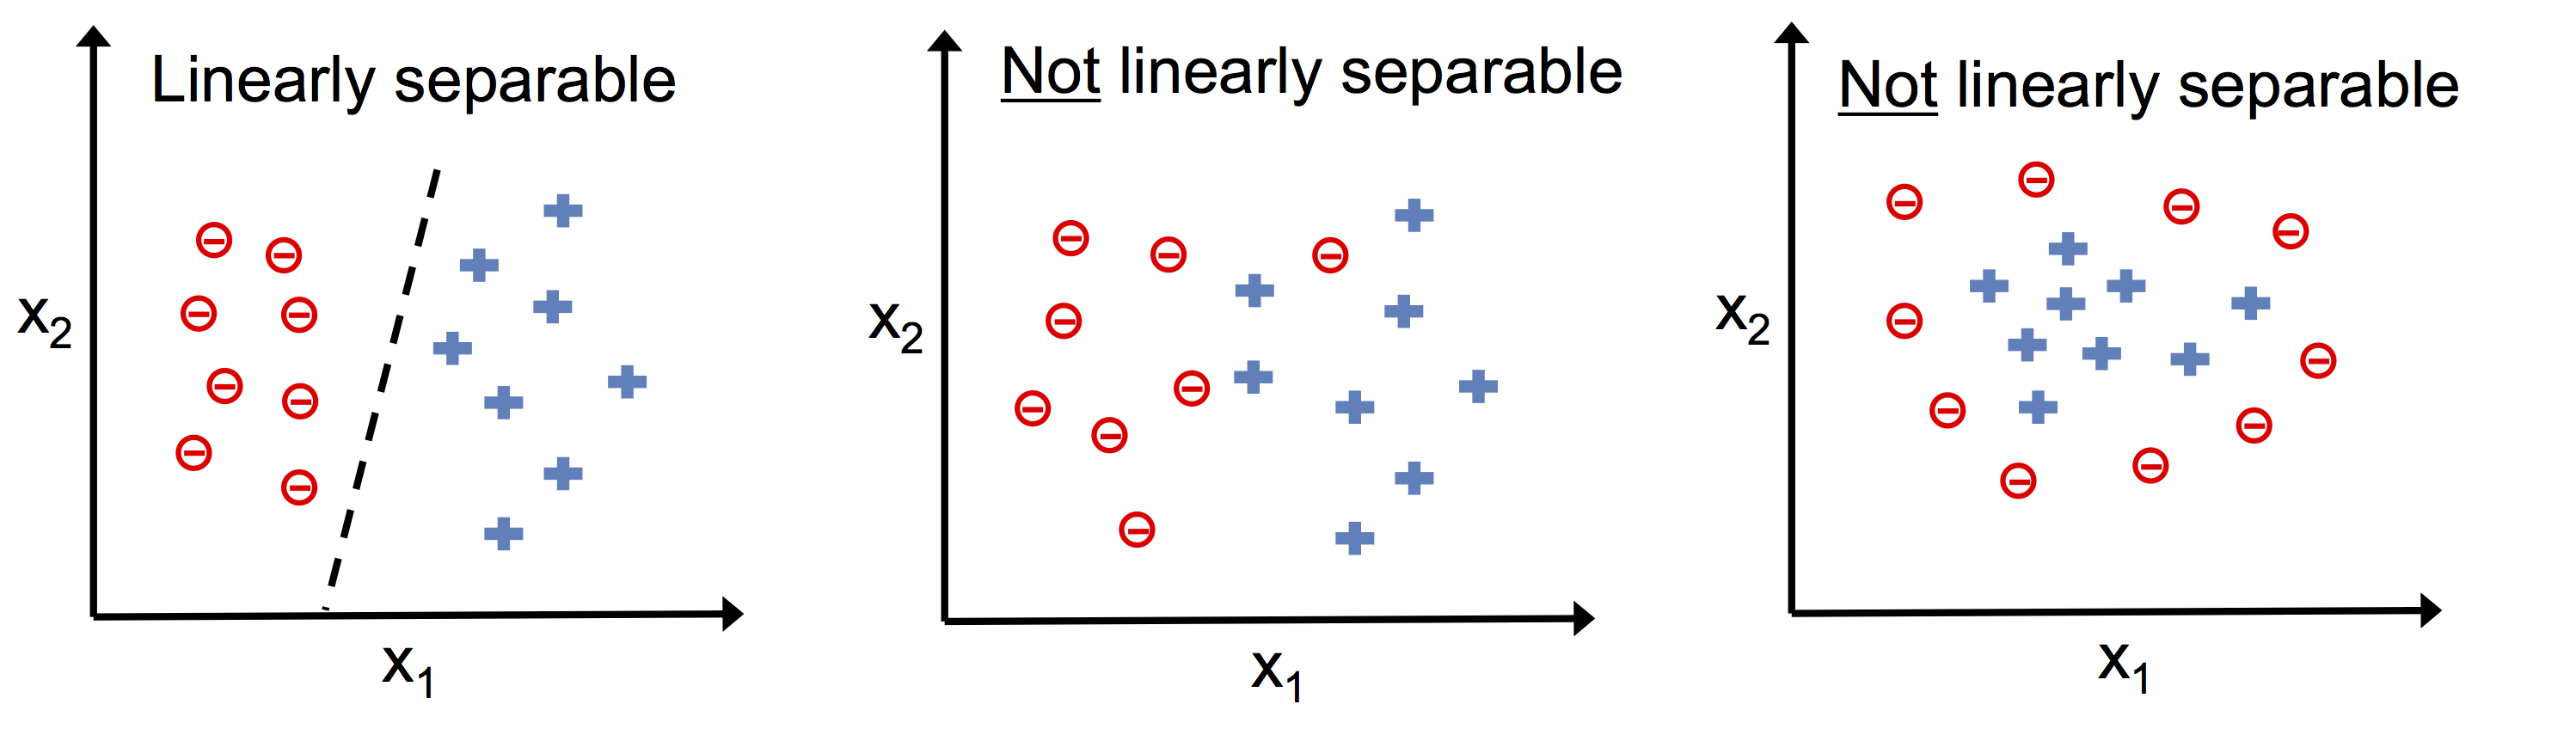
\includegraphics[width=\textwidth]{images/linearly_separable.png}
			\caption{Classes linéairement séparables \cite[image de][p. 48]{ml2008python}
			}
			\label{fig:linearly_separable}
		\end{figure}
	
	
		
		\subsubsection{Le modèle de la régression logistique} \label{subsec:reg_logistique}
		
		Ce qu'il est convenu d'appeler \textit{régression logistique} concerne en fait une méthode de classification binaire, à l'instar du perceptron (voir le point \ref{sec:perceptron}). A la différence du perceptron, cependant, nous allons chercher à apprendre une hypothèse $h$ définie de $\mathbb{R}^n$ dans [0,1], et non pas dans {0,1},  une motivation étant d'interpréter $h(x)$ comme étant la probabilité que l'entrée $x$ appartienne à la classe d'intérêt que nous notons $\mathcal{C}_1$. \cite{antoine2018apprentissage}
			
		Dans le cas à deux classes, nous sommes intéressés par le rapport de probabilités conditionnelles :
		\begin{equation}\label{eq:proba_cond}
			\frac{\mathbf{P}(y=\mathcal{C}_1|\mathbf{x})}{\mathbf{P}(y=\mathcal{C}_2|\mathbf{x})} = \frac{\mathbf{P}(y=\mathcal{C}_1)}{\mathbf{P}(y=\mathcal{C}_2)} \ \frac{\mathbf{p}(\mathbf{x}|y=\mathcal{C}_1)}{\mathbf{p}(\mathbf{x}|y=\mathcal{C}_2)}
		\end{equation}
		
		Bien entendu, on affecte l'entrée $x$ à la classe $\mathcal{C}_1$ si le rapport \ref{eq:proba_cond} est > 1, et à la classe $\mathcal{C}_1$ sinon \cite{antoine2018apprentissage}.
		
		
		Le terme $\frac{\mathbf{p}(\mathbf{x}|y=\mathcal{C}_1)}{\mathbf{p}(\mathbf{x}|y=\mathcal{C}_2)}$ est n'est facile à estimer à partir des fréquences mesurées des classes $\mathcal{C}_1$ et $\mathcal{C}_2$. Pour estimer ce terme, il faut faire des hypothèses sur sa forme.
		Dans la régression logistique, on fait l'hypothèse que le logarithme du rapport est de forme linéaire: 
			%log p(xly=w₁) P(xy= =w₂) S = w x + wo
		
		$$ 
		\log \left\lbrace \frac{\mathbf{p}(\mathbf{x}|y=\mathcal{C}_1)}{\mathbf{p}(\mathbf{x}|y=\mathcal{C}_2)} \right \rbrace  = w^Tx+b_0
		$$
		
		Il est possible de ré-exprimer l'équation \ref{eq:proba_cond} en utilisant les propriétés logarithmique, rappel :
		$$
		\log(a.b) = \log(a)+\log(b) \qquad log(x)^n = n\log(x) 
		$$
		et en utilisant la règle de Bayes, l'équation \ref{eq:proba_cond} deviendra :
		
		\begin{equation}\label{eq:re_proba_cond}
			\log\frac{\mathbf{P}(\mathcal{C}_1|\mathbf{x})}{1-\mathbf{P}(\mathcal{C}_1|\mathbf{x})} = \log\frac{\mathbf{P}(\mathcal{C}_1)}{\mathbf{P}(\mathcal{C}_2)} \ +\log\frac{\mathbf{p}(\mathbf{x}|y=\mathcal{C}_1)}{\mathbf{p}(\mathbf{x}|y=\mathcal{C}_2)} = w^Tx+b
		\end{equation}
		%\begin{figure}[bth]%bth
		%	\centering
			%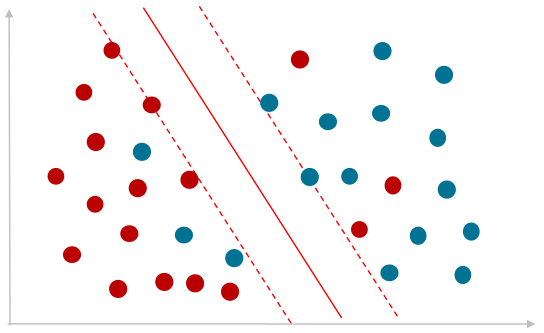
\includegraphics[width=8cm]{images/classification_minimisation.png}
			%\caption{Classification linéaire qui montre la zone de décision et la droite séparatrice.}
			%\label{fig:classification_zone}
		%\end{figure}
		
		%\begin{figure}[bth]%bth
		%	\centering
		%	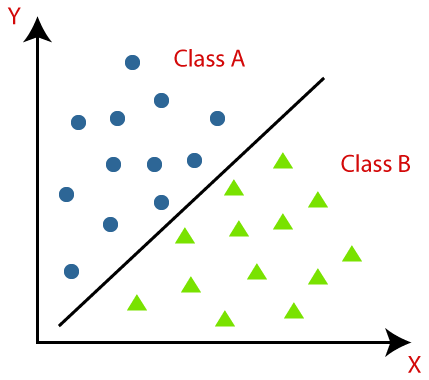
\includegraphics[width=8cm]{images/classification_linear.png}
		%	\caption{Classification linaire.}
			%\label{fig:classification_linear}
		%\end{figure}
	
		\begin{figure}[H]
			\myfloatalign
			\subfloat[La zone de décision et la droite séparatrice.]
			{\label{fig:classification_zone}
				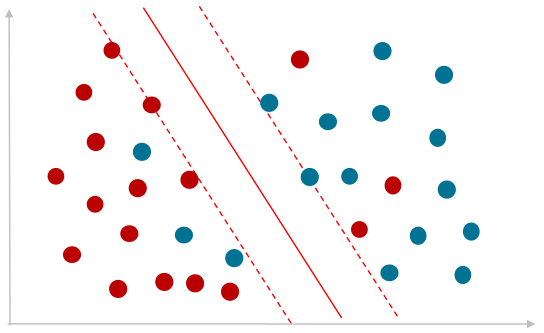
\includegraphics[width=.45\linewidth]{images/classification_minimisation.png}} \quad
			\subfloat[Classification linaire de deux classes A et B]
			{\label{fig:classification_linear}
				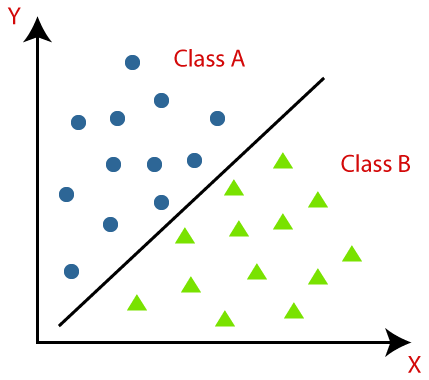
\includegraphics[width=.45\linewidth]{images/classification_linear.png}} 
			
			\caption{Exemple de la classification}\label{fig:classification_2case}
		\end{figure}
		\vspace*{3cm}
		La fonction de la droite séparatrice comme l'illustre la figure \ref{fig:classification_zone} et \ref{fig:classification_linear} s'écrit:
		\begin{equation}\label{eq:droite_sep}
			z = w _{1}x_{1}+\cdots +w_{n}x_{n}+b
		\end{equation}
		
		avec $ i=1,\ldots ,n,$ et $w_i$ et $b$ des paramètres de la droite.  %et $b = \varepsilon$
		\\
		$
		\begin{cases}
			\hat{y}=0 \ \ (y \in \mathcal{C}_1) & \quad \text{si  } z < 0\\
			\hat{y}=1 \ \ (y \in \mathcal{C}_2) & \quad \text{si  } z \geq 0
		\end{cases}
		$\\
		%??? changement de plan
		
		La fonction logistique est une fonction sigmoïde , qui prend n'importe quelle entrée réelle $t$, et renvoie une valeur comprise entre zéro et un \cite{ml2008python}. La fonction logistique standard ${\displaystyle \sigma :\mathbb {R} \rightarrow (0,1)}$ est défini comme suit :
		\begin{equation} \label{eq:sigmoid-simple}
		\sigma (t)={\frac {e^{t}}{e^{t}+1}}={\frac {1}{1+e^{-t}}}
		\end{equation}
		
		Supposons que $t$ est une fonction linéaire (comme la droite de la formule \ref{eq:droite_sep}) $t = z$. Et la fonction logistique générale ${ p:\mathbb {R} \rightarrow (0,1)}$ peut maintenant l'écrire :
		\begin{equation}\label{eq:sigmoid-dev}
			{\displaystyle p(x)=\sigma (z)= {\frac {1}{1+e^{-z}}} ={\frac {1}{1+e^{-(w _{1}x_{1}+\cdots +w_{n}x_{n}+b)}}}}
		\end{equation} 
		
		
		
		Dans le modèle logistique, $p(x)$ est interprété comme la probabilité de la variable dépendante ${Y}$ équivalant à un succès/cas-oui plutôt qu'à un échec/non-cas. Il est clair que les variables de réponse $Y_{i}$ ne sont pas identiquement répartis :$P(Y_{i}=1\mid X)$ diffère d'un point de données $X_{i}$ à l'autre, bien qu'ils soient indépendants étant donné la matrice de conception $X$ et paramètres partagés $w$ \cite{antoine2018apprentissage}. 
		
	
		\begin{figure}[H]%bth
			\centering
			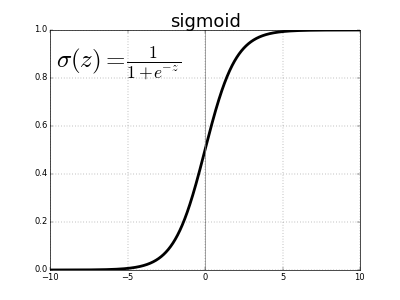
\includegraphics[width=10cm]{images/sigmoid_graph.png}
			\caption{Graphique représentant fonction sigmoïde logistique ajustée aux données $(x_n , y_n)$. \cite{ml2008python}
			}
			\label{fig:reg_log_sigmoid}
		\end{figure}
	
	\paragraph*{La vraisemblance:}Indique la plausibilité du  modèle vis-a-vis du vraies données.
	Soit l'échantillon $ \mathcal{S} = {(\mathbf{x}_1, y_1),..., (\mathbf{x}_m, y_m)}$, avec $y_i \in \{\mathcal{C}_1,\mathcal{C}_2\}, \forall_i \in (1,...,m)$. Sa vrai semblance en fonction des paramètres à apprendre s'écrit:
	
	\begin{equation}\label{eq:likelyhood}
		L = \prod_{i=1}^{m} {p_i}^{y_i} (1-p_i)^{1-y_i}
	\end{equation}
	
	où $m$ est le nombre d'exemples d'apprentissage appartenant à la classe.
	
	Dans \cite{antoine2018apprentissage}, il est montré que ces paramètres peuvent être obtenus par maximisation de la vraisemblance des paramètres conditionnellement aux exemples. Il a été de plus montré que, sous des conditions très générales \cite{sarkar2017practical}, le maximum de $L$ est unique.
	La maximisation de la vraisemblance se fait sois en passant par le logarithme, pour obtenir la log-vraisemblance :
	\begin{equation}
		\begin{split}
			\log(L)  & = \log(\prod_{i=1}^{m} {p_i}^{y_i} (1-p_i)^{1-y_i}) \\
			& =\sum_{i=1}^{m} \log( {p_i}^{y_i}) +\log((1-p_i)^{1-y_i})\\
			& =\sum_{i=1}^{m} {y_i}\log( {p_i}) +{(1-y_i)}\log(1-p_i)\\
		\end{split}
	\end{equation}
	Comme en Machine Learning on est plus apte à minimiser qu'à maximiser et Maximiser une fonction $f(\cdot)$ consiste à Minimiser $-f(\cdot)$ alors le log-vraisemblance s'écrira: 
	\begin{equation}\label{eq:log-likelyhood}
		\mathcal{L} = -\frac{1}{m}\sum_{i=1}^{m} {y_i}\log( {p_i}) +{(1-y_i)}\log(1-p_i)
	\end{equation}
	avec le terme $\frac{1}{m}$ pour augmenter la précision. Avec cette fonction, nous allons maximiser la vraisemblance $L$ en minimisant $-\log(L)$.	
		
	\pagebreak
	
\section{Réseau de neurones, apprentissage en profondeur}
	\begin{figure}[hth]%bth
		\centering
		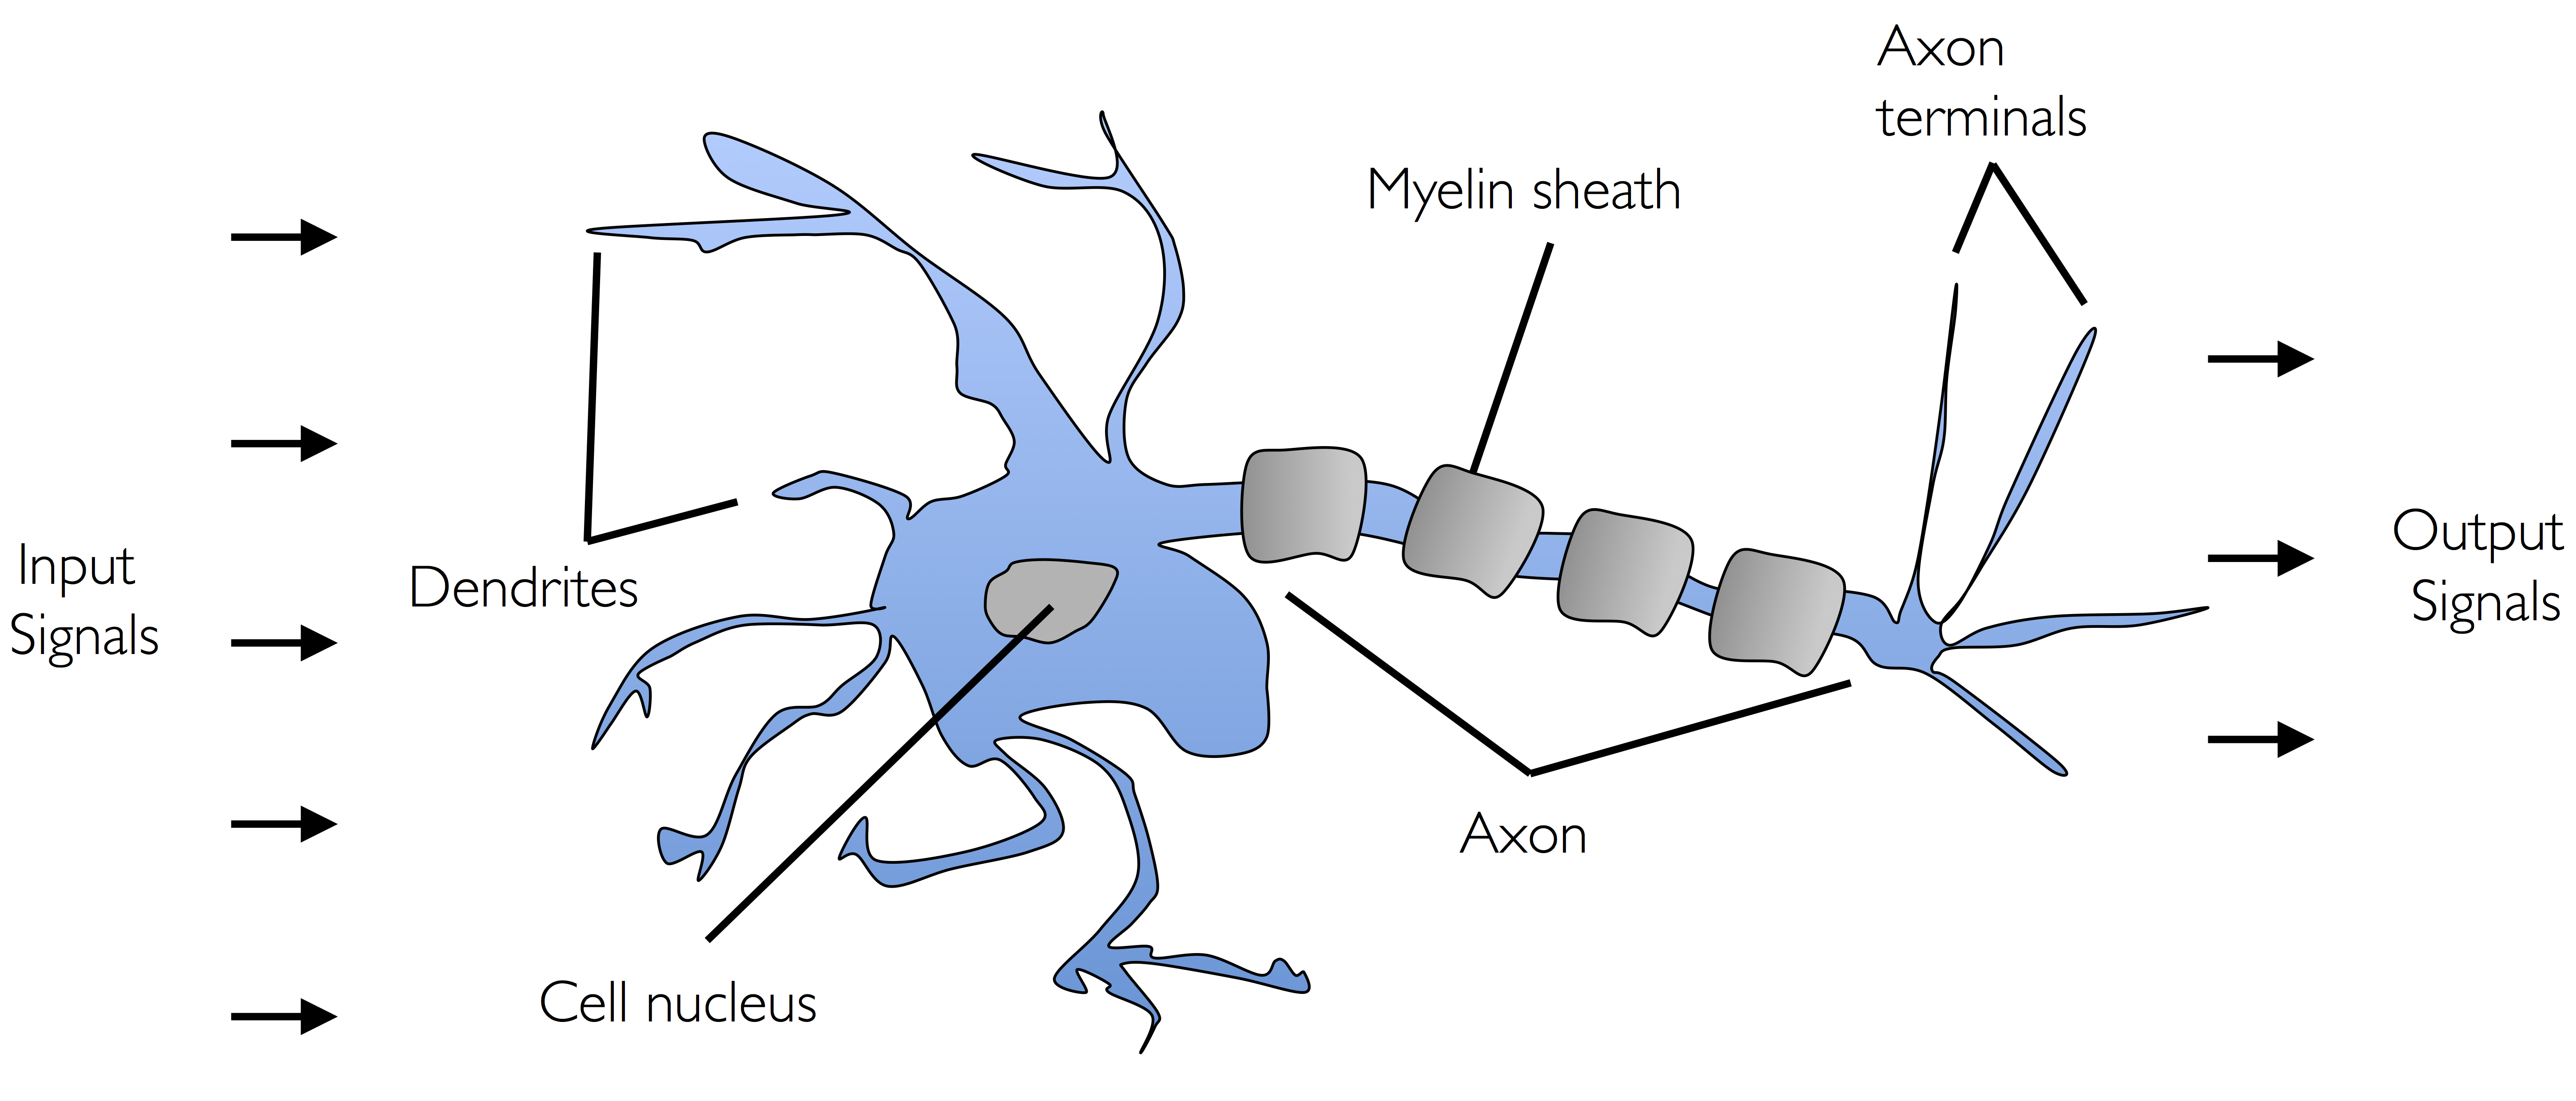
\includegraphics[width=\textwidth]{images/neuron.png}
		\caption{Neurone biologique \cite{ml2008python}}
		\label{fig:bio_neuron}
	\end{figure}


	\subsection{Perceptron} \label{sec:perceptron}
	
	Le perceptron est un modèle simplifié d'un neurone biologique. Alors que la complexité des modèles de neurones biologiques est souvent nécessaire pour bien comprendre le comportement neuronal, la recherche suggère qu'un modèle linéaire de type perceptron peut produire certains comportements observés dans de vrais neurones.
	
	Un perceptron est donc une unité de réseau neuronal, l'élément de traitement de base, qui effectue certains \textit{calculs} pour détecter des caractéristiques ou une intelligence économique dans les données d'entrée.\\ 
	Le perceptron, à l'instar du neurone artificiel classique, est conçu avec un algorithme d'apprentissage supervisé du même nom. %Un classificateur binaire est une fonction qui peut décider si une entrée, représentée par un vecteur de nombres, appartient ou non à une classe spécifique [??]. Il s'agit d'un type de classificateur linéaire , c'est-à-dire un algorithme de classification qui fait ses prédictions sur la base d'une fonction prédictive linéaire combinant un ensemble de poids avec le vecteur de caractéristiques.
	\begin{figure}[H]%bth
		\centering
		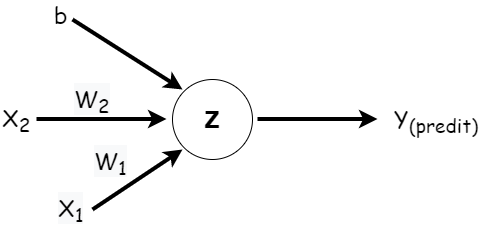
\includegraphics[width=9cm]{images/neuron-3-param.png}
		\caption{Neurone logique avec deux entrées $x_1$ et $x_2$ et les paramètres $w_1$, $w_2$ ($w_i$ dans un réseau de neurones il est nommé poids) et $b$ aussi appelé biais. le fonction d'agrégation $z$ (voir le point \ref{subsec:reg_logistique}, section \ref{sec:regression_problem}  et la formule \ref{eq:droite_sep})  sera: $z=w_1 x_1 +w_2 x_2 + b$.}
		\label{fig:logic_neuron}
	\end{figure}
	
	Le perceptron a des entrées qui peuvent provenir de l'environnement ou peuvent être les sorties d'autres perceptrons.
	Associé à chaque entrée, $ x_j \in \mathbb{R}$, avec $ j = 1,2, \dots , n, $ est un \textit{poids de connexion, ou poids} synaptique $w_j \in \mathbb{R}$, et la sortie, $\hat{y}$. Dans le cas le plus simple $\hat{y}$ est une somme pondérée des entrées \cite{alpaydin2010introduction}.
	
	$$ {\hat{y} = \sum _{j=1}^{n}w_{j}x_{j} + w_0} $$
	
	$w_0$ est la valeur d'interception pour rendre le modèle plus général, il est généralement modélisé comme la pondération provenant d'une unité de biais supplémentaire, $b = w_0 x_0$, avec $x_0$ qui est toujours égale $+1$. Nous pouvons écrire la sortie du perceptron sous la forme d'un produit scalaire.
	$$ \hat{y} = x^Tw $$
	
	Pendant le test, avec des poids donnés, $w$, pour l'entrée $x$, nous calculons la sortie $\hat{y}$. Pour implémenter une tâche donnée, nous avons besoin d'apprendre les poids $w$, les paramètres du système, de sorte que des sorties correctes soient générées compte tenu des entrées.
	
	\begin{figure}[hth]%bth
		\centering
		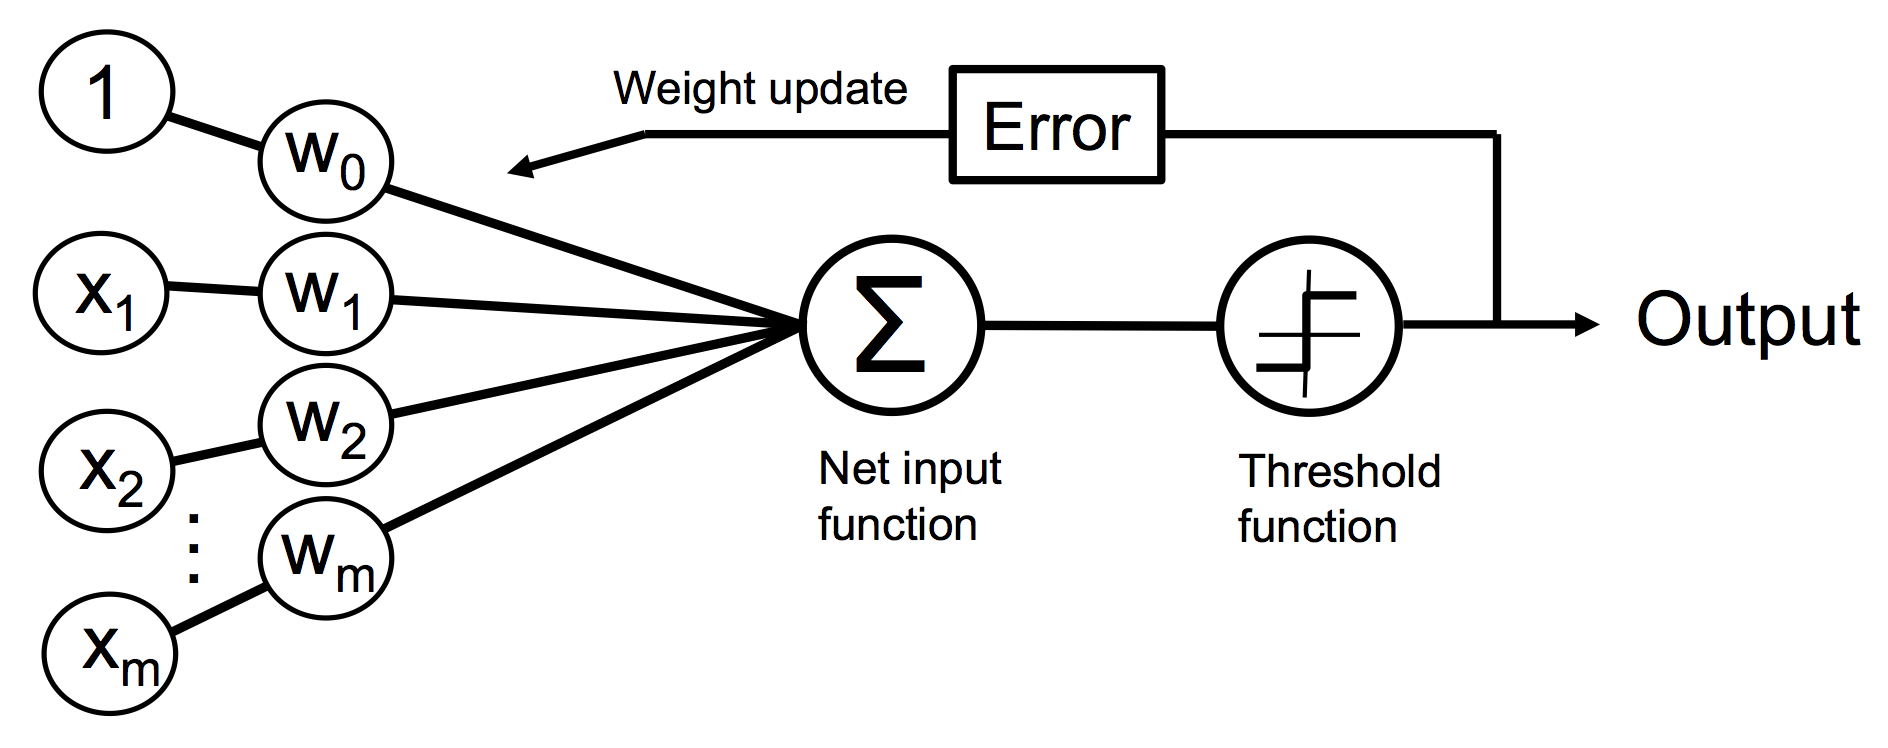
\includegraphics[width=\textwidth]{images/perceptron_neuron.png}
		\caption{Neurone artificiel modèle perceptron \cite{ml2008python}, cette figure est plus adapté pour représenter le modèle du perceptron.}
		\label{fig:perceptron_neuron}
	\end{figure}
	
	\subsubsection{Calcul avec l'algorithme du perceptron}
	
	Le premier concept de règle d'apprentissage du perceptron, a été publié par Frank Rosenblatt \cite{antoine2018apprentissage}, basé sur le modèle neuronal MP Neuron (McCulloch-Pitts Neuron). 
	
	%(F. Rosenblatt, The Perceptron, a Perceiving and Recognizing Automaton. Cornell Aeronautical Laboratory, 1957).
	
	Avec sa règle de perceptron, Il a proposé un algorithme qui apprendrait automatiquement les coefficients de poids optimaux qui sont ensuite multipliés par les caractéristiques d'entrée afin de décider si un neurone se déclenche ou non. Dans le cadre de l'apprentissage supervisé et de la classification, un tel algorithme pourrait alors être utilisé pour prédire si un échantillon appartient à une classe ou à l'autre \cite{ml2008python}.
	
	Il est important de noter que la convergence du perceptron n'est garantie que si les deux classes sont linéairement séparables et que le taux d'apprentissage est suffisamment faible. Si les deux classes ne peuvent pas être séparées par une limite de décision linéaire, nous pouvons définir un nombre maximum de passages sur l'ensemble de données d'apprentissage (époques) et/ou un seuil pour le nombre d'erreurs de classification tolérées - le perceptron n'arrêterait jamais de mettre à jour les poids autrement.
	
	???
	L'algorithme du perceptron travaille directement sur le vecteur a qui caractérise la surface discriminante cherchée. On n'a donc plus besoin ici de se placer dans l'espace de représentation de dimension d+1 ni d'utiliser le vecteur A. Cet algorithme utilise un protocole d'apprentissage itératif : il prend les données d'apprentissage les unes après les autres, chacune étant choisie soit par un passage systématique dans l'ensemble d'apprentissage (version « non stochastique »), soit par un tirage au hasard dans celui-ci (version « stochastique »). Son nombre d'étapes effectives peut être important: un seul (exactement ou en moyenne) passage des données n'est en effet pas suffisant pour le faire converger.
	
	???
	
	
	\begin{algorithm}[H]
		\caption{Perceptron, version stochastique}
		\begin{algorithmic} 
			\REQUIRE $n \geq 0 \vee x \neq 0$
			\STATE $t \leftarrow 0$
			
			\WHILE{$N \neq 0$}
				\STATE get random $x_i \in X$ set
				\IF{$x$ is classed}
					\STATE $a_{t+1} \leftarrow a_t$
				\ELSE[]
					\IF{$x \in \mathcal{W}_1$}
						\STATE	$a_{t+1} \leftarrow a_t + \alpha x$
					\ELSE[]
						\STATE	$a_{t+1} \leftarrow a_t - \alpha x$
					\ENDIF
					\STATE $t \leftarrow t + 1 $
	
				\ENDIF
			\ENDWHILE
			
			
			
		\end{algorithmic}
	\end{algorithm}
	

	\subsubsection{Le réseau de neurones artificiels (Perceptron Multicouche)}
	
	Les réseaux de neurones ont été introduits pour la première fois comme méthode d'apprentissage par Frank Rosenblatt, bien que le modèle d'apprentissage appelé perceptron soit différent des réseaux de neurones modernes, nous pouvons toujours considérer le perceptron comme le premier réseau de neurones artificiels \cite{sarkar2017practical}.

	Le perceptron multicouche (en anglais: multilayer perceptron MLP) est un type de réseau neuronal artificiel organisé en plusieurs couches, où les informations ne circulent que de la couche d'entrée à la couche de sortie. Il s'agit donc d'un réseau à propagation directe (feed forward), autrement dit le réseau profond à action directe. Un perceptron multicouche est juste une fonction mathématique mappant un ensemble de valeurs d'entrée à des valeurs de sortie. La fonction est formée en composant de nombreuses fonctions plus simples. Nous pouvons considérer chaque application d'une fonction mathématique différente comme fournissant une nouvelle représentation de l'entrée \cite{goodfellow2016deep,antoine2018apprentissage}.
	
	Les perceptrons à une seule couche ne sont capables d'apprendre que des motifs linéairement séparables. Pour une tâche de classification avec une fonction d'activation d'étape, un seul nœud aura une seule ligne divisant les points de données formant les motifs. Plus de nœuds peuvent créer plus de lignes de division, mais ces lignes doivent en quelque sorte être combinées pour former des classifications plus complexes. Une deuxième couche de perceptrons, voire de nœuds linéaires, suffit à résoudre de nombreux problèmes autrement non séparables \cite{antoine2018apprentissage}.
	
	Les réseaux de neurones artificiels (ANN) fonctionnent vaguement sur le principe de l'apprentissage d'une distribution distribuée de données.
	L'hypothèse sous-jacente est que les données générées sont le résultat d'une combinaison non linéaire d'un ensemble de facteurs latents et si nous sommes capables d'apprendre cette représentation distribuée, nous pouvons alors faire des prédictions précises sur un nouvel ensemble de données inconnues. Le réseau de neurones le plus simple aura une couche d'entrée, une couche cachée (résultat de l'application d'une transformation non linéaire aux données d'entrée) et une couche de sortie. Les paramètres du modèle ANN sont les poids de chaque connexion qui existent dans le réseau et parfois un paramètre de biais \cite{sarkar2017practical}.
	
	
	
	\begin{figure}[hth]%bth
		\centering
		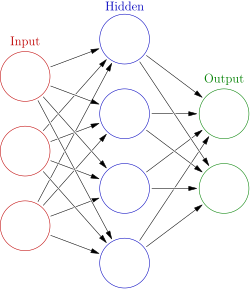
\includegraphics[width=6cm]{images/colored_neural_network.png}
		\caption{Un réseau de neurones artificiels est un groupe de nœuds inter-connectés, inspiré d'une simplification des neurones d'un cerveau. Ici, chaque nœud circulaire représente un neurone artificiel et une flèche représente une connexion de la sortie d'un neurone artificiel à l'entrée d'un autre.}
		\label{fig:colored_neural_network}
	\end{figure}
	
	\subsection{Fonctions d'activation, poids et biais} \label{sec:activation_weight}
	
	%\subsubsection{Poids et biais}
	
	\subsubsection{Fonctions d'activation tangente (Sigmoïde et  hyperbolique)}
	La fonction d'activation est responsable de la transformation de l'entrée pondérée sommée du nœud en activation du nœud ou de la sortie pour cette entrée.
	Pour un nœud donné, les entrées sont multipliées par les poids d'un nœud et additionnées. Cette valeur est appelée activation sommée du nœud. L'activation sommée est ensuite transformée via une fonction d'activation et définit la sortie spécifique ou « activation » du nœud \cite{ml2008python}.\\
	La fonction sigmoïde (aussi appelé fonction logistique voir le point \ref{sec:classificarion_problem} \ref{subsec:reg_logistique}) est utilisée ici comme une fonction d'activation.	
	
	La fonction d'activation la plus simple est appelée activation linéaire, où aucune transformation n'est appliquée. Un réseau composé uniquement de fonctions d'activation linéaires est très facile à former, mais ne peut pas apprendre des fonctions de cartographie complexes. Les fonctions d'activation linéaires sont toujours utilisées dans la couche de sortie pour les réseaux qui prédisent une quantité (par exemple, les problèmes de régression, voir le point \ref{sec:regression_problem}) \cite{geron2017hands, krizhevsky2012imagenet}.
	
	Les fonctions d'activation non linéaires sont préférées car elles permettent aux nœuds d'apprendre des structures plus complexes dans les données. Traditionnellement, deux fonctions d'activation non linéaires largement utilisées sont les fonctions d'activation tangente sigmoïde et hyperbolique \cite{goodfellow2016deep}.
	
	La fonction \textbf{d'activation sigmoïde}, est traditionnellement une fonction d'activation très populaire pour les réseaux de neurones. L'entrée de la fonction est transformée en une valeur comprise entre $0,0$ et $1,0$. Les entrées qui sont beaucoup plus grandes que $1,0$ sont transformées à la valeur $1,0$, de même, les valeurs beaucoup plus petites que $0,0$ sont alignées sur $0,0$. La forme de la fonction pour toutes les entrées possibles est une forme en S de zéro jusqu'à 0,5 à 1,0. Pendant longtemps, jusqu'au début des années 1990, c'était l'activation par défaut utilisée sur les réseaux de neurones \cite{krizhevsky2012imagenet}.
	
	
	La fonction \textbf{tangente hyperbolique}, ou \textbf{tanh} en abrégé, est une fonction d'activation non linéaire de forme similaire qui génère des valeurs comprises entre -1,0 et 1,0. À la fin des années 1990 et au cours des années 2000, la fonction tanh a été préférée à la fonction d'activation sigmoïde car les modèles qui l'utilisaient étaient plus faciles à entraîner et avaient souvent de meilleures performances prédictives \cite{goodfellow2016deep}.
	la fonction d'activation tangente hyperbolique fonctionne généralement mieux que la sigmoïde logistique.
	\subsubsection*{Limitations des fonctions d'activation sigmoïde et tanh}
	Cela signifie que pour tanh et sigmoïde, les grandes valeurs sont alignées sur 1,0 et les petites valeurs sont alignées sur -1 ou 0. De plus, la fonction n'est vraiment sensible qu'aux changements proches du point médian de l'entrée. Par exemple, 0,5 pour les sigmoïdes et 0,0 pour la tanh.
	
	 Les unités sigmoïdales saturent sur la majeure partie de leur domaine - elles saturent à une valeur élevée lorsque z est très positif, saturent à une valeur faible lorsque z est très négatif et ne sont fortement sensibles à leur entrée que lorsque z est proche de 0 \cite{ml2008python}.
	 
	 La sensibilité et la saturation limitées de la fonction se produisent indépendamment du fait que l'activation additionnée du nœud fourni en entrée contient des informations utiles ou non. Une fois saturé, il devient difficile pour l'algorithme d'apprentissage de continuer à adapter les poids pour améliorer les performances du modèle.
	 
	 Les couches profondes des grands réseaux utilisant ces fonctions d'activation non linéaires ne reçoivent pas d'informations de gradient utiles. L'erreur est rétropropagée (voir le point ???) sur le réseau et utilisée pour mettre à jour les pondérations. La quantité d'erreur diminue considérablement avec chaque couche supplémentaire à travers laquelle elle se propage, compte tenu de la dérivée de la fonction d'activation choisie. C'est ce qu'on appelle le problème du gradient de fuite et empêche les réseaux profonds (multicouches) d'apprendre efficacement \cite{geron2017hands}.
	 
	 Bien que l'utilisation de fonctions d'activation non linéaires permette aux réseaux de neurones d'apprendre des fonctions de cartographie complexes, elles empêchent efficacement l'algorithme d'apprentissage de fonctionner avec des réseaux profonds.
	 
	
	
	\subsubsection{Fonction d'activation ReLU}
	
	Dans le domaine des réseaux de neurones artificiels, ReLU (Rectified Linear Unit) ou fonction d'activation du redresseur est une fonction d'activation définie comme la partie positive de son argument \cite{goodfellow2016deep}.
	$${\displaystyle f(x)=x^{+}=\max(0,x)}$$
	ReLU est une fonction linéaire par morceaux qui produira l'entrée directement si elle est positive, sinon, elle produira zéro. C'est devenu la fonction d'activation par défaut pour de nombreux types de réseaux de neurones, car un modèle qui l'utilise est plus facile à former et atteint souvent de meilleures performances \cite{geron2017hands}.
	
	
	La conception d'unités cachées est un domaine de recherche extrêmement actif et ne dispose pas encore de nombreux principes directeurs théoriques définitifs.
	Les fonctions d'activations ReLU sont un excellent choix par défaut d'unité cachée. De nombreux autres types d'unités cachées sont disponibles. Il peut être difficile de déterminer quand utiliser quel type, bien que les unités linéaires rectifiées soient généralement un choix acceptable \cite{goodfellow2016deep}.
	
	???
	
	Pour un exemple de la façon dont ReLU peut résoudre le problème des gradients de fuite, consultez le didacticiel 


	%	\subsection{Neurones}
	%\lipsum[1]
	%\subsubsection{Réseau des neurones}
	
	
	\subsection{Réseau neuronal convolutif (CNN)}
	
	Le réseau neuronal convolutif est un type de réseau neuronal artificiel qui utilise plusieurs perceptrons qui analysent les entrées d'image et ont des poids et des bases apprenables sur plusieurs parties d'images et capables de se séparer les unes des autres \cite{tammina2019transfer}.
	
	Un réseau de neurones convolutifs (CNN, Convolutional Neural Network ou ConvNet) est un type de réseau de neurones artificiels acyclique à propagation avant, dans lequel le motif de connexion entre les neurones est inspiré par le cortex visuel des animaux. Les neurones de cette région du cerveau sont arrangés de sorte à ce qu'ils correspondent à des régions (appelés champs réceptifs) qui se chevauchent lors du pavage du champ visuel. Ils sont de plus organisés de manière hiérarchique, en couches (aire visuelle primaire V1, secondaire V2, puis aires V3, V4, V5 et V6, gyrus temporal inférieur), chacune des couches étant spécialisée dans une tâche, de plus en plus abstraite \cite{antoine2018apprentissage}. En simplifiant à l'extrême, une fois que les signaux lumineux sont reçus par la rétine et convertis en potentiels d'action:
	\begin{itemize}
		\item L'aire primaire V1 s'intéresse principalement à la détection de contours, ces contours étant définis comme des zones de fort constrate de signaux visuels re
	\end{itemize}
	
	???
	
	L'un des avantages de l'utilisation du réseau de neurones convolutifs est qu'il exploite l'utilisation de la cohérence spatiale locale dans les images d'entrée, ce qui leur permet d'avoir moins de poids car certains paramètres sont partagés \cite{tammina2019transfer}.
	
	
	???
	\cite{shin2016deep} 
	
	\subsubsection{La convolution}
	
	La convolution est une opération mathématique simple généralement utilisée pour le traitement et la reconnaissance d’images. Sur une image, son effet s’assimile à un filtrage dont voici le fonctionnement
	
	??? 
	
	\subsubsection{Les différents couches d'un CNN}
	???
	
	\subsubsection{L'architecture VGGNet}
	
	VGG signifie Visual Geometry Group, il s'agit d'une architecture standard de réseau de neurones à convolution profonde (CNN) à plusieurs couches. %Le "profond" fait référence au nombre de couches avec VGG-16 ou VGG-19 composé de 16 et 19 couches convolutionnelles.
	
	???
	
	Les réseaux VGG (Visual Geometry Group, université d'Oxford) [SZ14] ont été les premiers à utiliser de petits filtres de convolution (3×3) et à les combiner pour décrire des séquences de convolution, l'idée étant d'émuler l'effet de larges champs réceptifs par cette séquence. Cette technique amène malheureusement à un nombre exponentiel de paramètres (le modèle entraîné qui peut être téléchargé a une taille de plus de 500 Mo). VGG a concouru à ILSVRC 2014, a obtenu un taux de bonne classification de 92.3 \% mais n'a pas remporté le concours. Aujourd'hui, VGG est une famille de réseaux profonds (de A à E) qui varient par leur architecture (figure 10.9). Le nombre de paramètres (en millions) pour les réseaux de A à E est 133, 133, 134, 138 et 144. Les réseaux VGG-D et VGG-E sont les plus précis et populaires.???
	
	
	
	L'architecture VGG est  la base d'un modèle innovant de reconnaissance d'objets. Développé en tant que réseau neuronal profond, VGGNet va au-delà d'ImageNet et dépasse la ligne de base  de nombreuses tâches et ensembles de données. De plus, c'est toujours l'une des architectures de reconnaissance d'images les plus populaires \cite{tammina2019transfer, antoine2018apprentissage}.
	
	Les VGGNet sont basés sur les caractéristiques les plus essentielles des réseaux de neurones convolutifs (CNN). Le graphique suivant montre le concept de base du fonctionnement d'un CNN.
	
	
	\begin{list}{--}{Un bref coup d'œil à l'architecture de VGG :}
		\item \textbf{Entrée} : Le VGGNet prend une taille d'entrée d'image de 224×224. Pour le concours ImageNet, les créateurs du modèle ont recadré le patch central 224 × 224 dans chaque image pour conserver la cohérence de la taille d'entrée de l'image \cite{simonyan2014very}.
		
		\item \textbf{Couches convolutives }: Les couches convolutives de VGG tirent parti d'un champ de réception minimal, c'est-à-dire 3 × 3, la plus petite taille possible qui capture toujours haut/bas et gauche/droite. De plus, il existe également des filtres de convolution 1 × 1 agissant comme une transformation linéaire de l'entrée. Vient ensuite une unité ReLU, qui est une énorme innovation d'AlexNet qui réduit le temps de formation. ReLU signifie fonction d'activation d'unité linéaire rectifiée ; c'est une fonction linéaire par morceaux qui produira l'entrée si elle est positive ; sinon, la sortie est nulle. La foulée de convolution est fixée à 1 pixel pour conserver la résolution spatiale préservée après la convolution (la foulée est le nombre de décalages de pixels sur la matrice d'entrée) \cite{krizhevsky2012imagenet,tammina2019transfer}.
		
		\item \textbf{Couches cachées} : Toutes les couches cachées du réseau VGG utilisent ReLU. VGG n'utilise généralement pas la normalisation de la réponse locale (LRN) car elle augmente la consommation de mémoire et le temps de formation. De plus, il n'apporte aucune amélioration à la précision globale \cite{tammina2019transfer}.
		
		\item \textbf{Couches entièrement connectées} : Le VGGNet a trois couches entièrement connectées. Sur les trois couches, les deux premières ont 4096 canaux chacune et la troisième a 1000 canaux, 1 pour chaque classe \cite{tammina2019transfer}.
	
	\end{list}
	%------------------------------------------------------------------------------
	%\cite{simonyan2014very}
	%\cite{shin2016deep} 
	%\cite[ReLU]{pretorius2018critical}
	%------------------------------------------------------------------------------
	

	\begin{figure}[hth]%bth
		\centering
		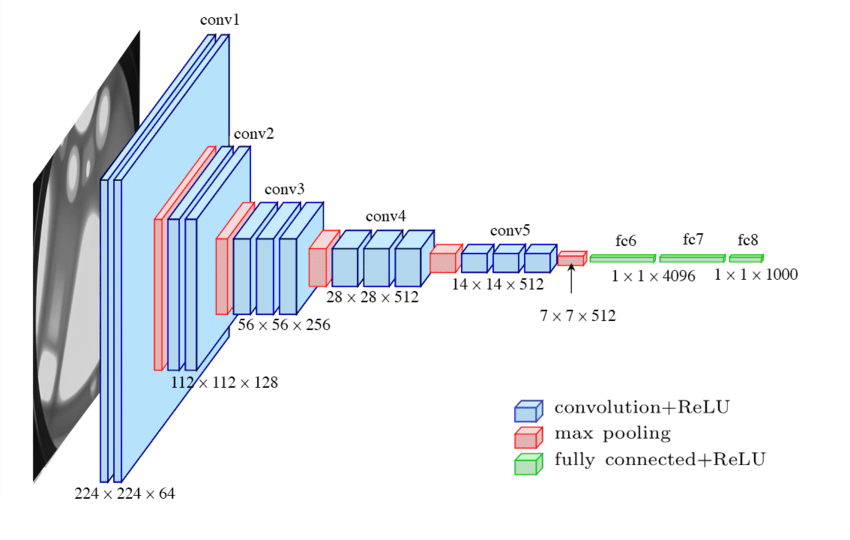
\includegraphics[width=\textwidth]{images/VGG-16-network-architecture.png}
		\caption{CNN : architecture VGG-16 \cite{ml2008python}
		}
		\label{fig:VGG16_network}
	\end{figure}
	
	
	%\subsubsection{Réseau neuronal récurrent (RNN)}
	%\lipsum[1]
	
	%\section{Réseaux de neurones}
	
	
	
	%\section{Classificateurs}
	%\lipsum[1]
	

		